\section{Reflection cancellation and global localization}
\label{sec:argmax}

The proof of Theorem~\ref{thm:main-location} compares every point with
the exact corner value $\Lambda_c(n)=\lambda_n(-1,-1)$.  A periodic
majorant provides one common comparison for all mesh cells.  Its
triangle-inequality loss distinguishes an interior mesh vertex from an
actual corner.  This loss compensates the growth of the majorant near the origin.

Put $m=n+1$ and $\mathsf N=nm$, and recall the finite angular kernel
$G_n$ from \eqref{eq:angular-kernel}, whose highest first-coordinate
coefficient is one. In this section the node angles
$\theta_j,\phi_k$ are written $a_j,b_k$ to distinguish them from
phase and row-profile arguments; the endpoint weights keep the
notation $\varepsilon_j,\eta_k$ of Section~\ref{sec:preliminaries}. Write
$a_j=j\pi/n$, $b_k=k\pi/m$, and let $\varepsilon_j,\eta_k$ equal one at interior
indices and $1/2$ at endpoints.  Product to sum in the cardinal formula gives
\begin{equation}\label{ul:cardinal-reflection}
 L_{jk}(\cos\theta,\cos\phi)=\frac{w_{jk}}4
   \sum_{\sigma,\eta=\pm1}G_n(\theta+\sigma a_j,\phi+\eta b_k),
 \qquad w_{jk}=\frac{2\varepsilon_j\eta_k}{\mathsf N}.
\end{equation}
For evaluation, with $P_n=T_{n+1}+T_n$, one may equivalently use
$G_n(u,v)=[P_n(\cos u)-P_n(\cos v)]/(\cos u-\cos v)-\cos(nu)$.
A collision means equality of the two cosine arguments. At a collision this means the polynomial divided difference, including
$P_n'(\cos u)$ at equality.  Every formula below includes these values.

Use odd mesh charts
\begin{equation}\label{ul:charts}
 \theta=(J\pi+\alpha)/n,\quad \phi=(K\pi+\beta)/m,
 \quad J+K\text{ odd},\quad |\alpha|+|\beta|\leq\pi,
 \quad (\theta,\phi)\in[0,\pi]^2,
\end{equation}
where $0\leq J\leq n$, $0\leq K\leq m$.  These cover the closed
square: in each angular mesh rectangle, the distances in mesh-index units to its
two odd vertices sum to two, so one is at most one; multiplying by
$\pi$ gives the phase radius in \eqref{ul:charts}.  The chart center is the mesh point $(J\pi/n,K\pi/m)$. Put
$x=|\alpha|$, $y=|\beta|$ and $\rho=x+y$.
The signed diamond is $|\alpha|+|\beta|\leq\pi$; its folded
phase triangle is $x,y\geq0$, $x+y\leq\pi$.
A point on a tie belongs to every chart it satisfies.
Set $\Gamma^-=\{(r,s):0\leq r<2n,\ 0\leq s<2m,\ r+s\text{ odd}\}$ and
\begin{equation}\label{ul:primitive}
 H_{rs}=G_n((r\pi+\alpha)/n,(s\pi+\beta)/m),\qquad
 S_n(\alpha,\beta)=\frac1{2\mathsf N}\sum_{\Gamma^-}|H_{rs}|.
\end{equation}
The endpoint identity
$\sum_{\sigma=\pm1}\sum_{0\leq j\leq n,\,\sigma j\equiv r\ (2n )}\varepsilon_j=1$
and its $m$ counterpart give total weight one at every periodic
index: the two endpoint preimages have half weights, while an interior
index has one preimage of weight one. The two-coordinate weights
factorize, and their parity is $j+k$ even exactly when $r+s$ is odd
in the shifted odd chart. Thus summing the four absolute reflected
terms in \eqref{ul:cardinal-reflection} gives exactly $S_n$.
Consequently, with $g_{\sigma\eta}=G_n(\theta+\sigma a_j,\phi+\eta b_k)$,
\begin{equation}\label{ul:defect}
 \lambda_n=S_n-\Delta_{JK},\qquad
 \Delta_{JK}=\sum_{j+k\,\mathrm{even}}\frac{w_{jk}}4
 \left(\sum_{\sigma,\eta}|g_{\sigma\eta}|
             -\left|\sum_{\sigma,\eta}g_{\sigma\eta}\right|\right)\geq0.
\end{equation}
For $\mathfrak d(z,w)=|z|+|w|-|z+w|$, periodic indices give the two projections
\begin{equation}\label{ul:projections}
 Q_v(K)=\frac1{4\mathsf N}\sum_{\Gamma^-}\mathfrak d(H_{rs},H_{r,2K-s}),
 \qquad
 Q_h(J)=\frac1{4\mathsf N}\sum_{\Gamma^-}\mathfrak d(H_{rs},H_{2J-r,s}).
\end{equation}
Pairing first in either coordinate proves
$\Delta_{JK}\geq\max(Q_h,Q_v)$.
At an actual nonnode corner all four reflected values coincide, so
$\Delta=0$ and $S_n(0,0)=\Lambda_c(n)$.
Separate phase reflections and translations by the even lattice preserve
$S_n$.  Reducing each phase modulo $2\pi$ and, if necessary, using
$(x,y)\mapsto(\pi-x,\pi-y)$ reduces its global real-phase norm, the supremum of $S_n$ over
$(\alpha,\beta)\in\mathbb R^2$, to
$x,y\geq0$, $x+y\leq\pi$.  Throughout, $x$ refers to the $n$-mesh and $y$ to the $m$-mesh.


At $(-1,-1)$, inward phases $A,B\geq0$ parameterize
$(-\cos(A/n),-\cos(B/m))$; the other nonnode corner uses its parity reflection.

\begin{center}\small
\begin{tabular}{@{}ll@{}}\toprule
Symbols & Meaning\\\midrule
$m=n+1$, $\mathsf N=nm$ & adjacent mesh size and product size\\
$a_j,b_k$; $\varepsilon_j,\eta_k$ & node angles and endpoint weights\\
$J,K$; $\alpha,\beta$; $x,y,\rho$ & chart center indices; signed and folded phases; radius\\
$\Gamma^-,H_{rs},S_n$ & odd periodic indices, kernel samples, absolute envelope\\
$\Delta_{JK}$; $\mathfrak d,Q_h,Q_v$ & reflection loss; pair defect and its projections\\
$P_n=T_{n+1}+T_n$ & polynomial for the divided-difference kernel\\
$A,B$ & nonnegative inward corner phases\\\bottomrule
\end{tabular}
\end{center}

The organizing identity is
\[
 \lambda_n-\Lambda_c=(S_n-S_n(0,0))-\Delta_{JK}.
\]
The model comparison bounds the first bracket; selected reflected
pairs give a positive lower bound for the second. After the comparison
theorem, two scalar gates and one corner lemma complete the analytic
argument. Here $A,B\geq0$ denote inward corner phases, so near $(-1,-1)$
the physical point is $(-\cos(A/n),-\cos(B/m))$.
The absolute gate $\mathcal G$ and relative quadratic $\mathfrak p_n$
are defined in Corollaries~\ref{uc:absolute-gate}--\ref{uc:relative-gate}.
Figure~\ref{fig:phase-regions} shows their domains. Their roles are:
\[
\begin{array}{llll}
\text{phase region}&\text{center}&\text{comparison}&\text{degree}\\
\rho\leq1/2&\text{noncorner}&\lambda_n<\Lambda_c-9/1000&n\geq512\\
1/2\leq\rho\leq1&\text{all}&S_n<\Lambda_c-1/7&n\geq512\\
1\leq\rho\leq\pi&\text{all}&S_n<\Lambda_c-1/2&n\geq512\\
0\leq A,B\leq\pi/4&\text{corner}&
 \lambda_n\leq\Lambda_c-(A^2+B^2)/30&n\geq256.
\end{array}
\]
The earlier far-region instance $n\geq192$, $\rho\geq\pi/2$ is
used only by the finite certificates in Section~\ref{sec:certificates}.

\begin{figure}[ht]
\centering
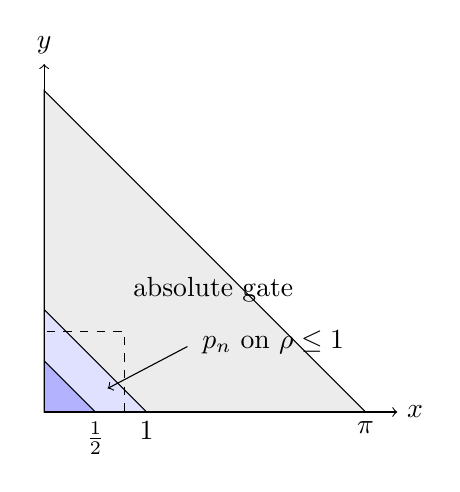
\begin{tikzpicture}[scale=1.3]
 \fill[gray!15] (0,1)--(1,0)--(3.14,0)--(0,3.14)--cycle;
 \fill[blue!12] (0,.5)--(.5,0)--(1,0)--(0,1)--cycle;
 \fill[blue!30] (0,0)--(.5,0)--(0,.5)--cycle;
 \draw (0,0)--(3.14,0)--(0,3.14)--cycle;
 \draw (.5,0)--(0,.5) (1,0)--(0,1);
 \draw[dashed] (0,0) rectangle (.7854,.7854);
 \draw[->] (0,0)--(3.45,0) node[right] {$x$};
 \draw[->] (0,0)--(0,3.4) node[above] {$y$};
 \node[below] at (.5,0) {$\frac12$};
 \node[below] at (1,0) {$1$};
 \node[below] at (3.14,0) {$\pi$};
 \node at (1.65,1.20) {absolute gate};
 \node[anchor=west] at (1.45,.68) {$\mathfrak p_n$ on $\rho\leq1$};
 \draw[->] (1.40,.64)--(.62,.23);
\end{tikzpicture}
\caption{The folded phase triangle. On the darkest triangle a
noncorner chart uses $\Delta>1/20$ together with $\mathfrak p_n$.
On $1/2\leq\rho\leq1$, $\mathfrak p_n<0$ suffices; the absolute gate covers
$\rho\geq1$. In a corner chart the dashed $\pi/4$ square has a
separate descent estimate.}
\label{fig:phase-regions}
\end{figure}

\subsection{A completed comparison model}
\label{uc:model}

Throughout the comparison argument $m=n+1$, $L=\log n$, $\bar{L}=1+L$,
$H_n=\sum_{j=1}^n j^{-1}$, and
\[
 \begin{gathered}
 x=|\alpha|,\quad y=|\beta|,\quad \rho=x+y\leq\pi,\quad
 c_e=\cos(\rho/2),\quad c_d=\cos((x-y)/2),\\
 \mathsf{a}=c_ec_d,\quad u=1-\mathsf{a},\quad z=(1-c_e)(1-c_d).
 \end{gathered}
\]
For a real number $t$, write $t_+=\max(t,0)$.
Also put $p=\sin x$, $q=\sin y$, $P=p+q$, and $d_+=(q-p)_+$.
Thus $\mathsf{a}=(\cos x+\cos y)/2\geq0$ and $2-c_e-c_d=u+z$.
Throughout, $x$ refers to the $n$-mesh and $y$ to the $m$-mesh.
A phase point is denoted $\varphi=(x,y)$.
For real $C,D$ and $0<e<\pi$, define the complete cancellation
\begin{align}\label{uc:cancellation}
 I(C,D,e)&=\int_0^\pi
 \{|C\cot t+D\cot(t+e)|-|C\cot t|-|D\cot(t+e)|\}\,dt,\notag\\
 J(v,s,e)&=I((v-s)/2,(v+s)/2,e).
\end{align}
Write $g(C,D;t)$ for this integrand, with the separation understood.
We integrate the combined integrand, whose pole limits are finite.
It is invariant under simultaneous coefficient reversal and exchange of
channels. The separation is even and $\pi$-periodic, so reduction to
$0<e\leq\pi/2$ covers every nonzero separation. At $e\equiv0$,
opposite coefficients may give a logarithmic divergence. In the row
profile below this is the integrable central logarithm at $v=\pi$.

\begin{lemma}[Cancellation and root formulas]\label{uc:cancellation-lemma}
For $v,s\geq0$, $0<e\leq\pi/2$, write
\[
 J(v,s,e)=2(s-v)_+\log\sin e+R(v,s,e).
\]
Then $R\leq0$,
\begin{align}\label{uc:R-bounds}
 |R|&\leq\max(2v,s+v)\log2,
 &|R_s|&\leq\log\frac{v+s}{|v-s|},\\
 R_e&=\frac{2\{v\cos e-\sqrt{(v^2-s^2\sin^2e)_+}\}}{\sin e}
 &&(s>v),\qquad R_e=0\quad(s\leq v).\notag
\end{align}
The derivative in $s$ is used as a locally integrable bound at $s=v$.
If
\begin{equation}\label{uc:root-Z}
 E(v,s,e)=J(v,s,e)-2s\log\sin e,\qquad
 Z(v,s,e)=2\int_e^{\pi/2}
       \frac{\sqrt{(v^2-s^2\sin^2t)_+}}{\sin t}\,dt,
\end{equation}
then $E\leq Z$, with equality for $s\geq v$.
All complete formulas extend continuously through zero coefficients
and moving equality roots.
\end{lemma}
\begin{proof}
On a sign interval the integrand is $-2$ times the smaller absolute
channel, and its primitive is a linear combination of logarithms of
sines. For $s\leq v$, with $c=(v-s)/2$, $b=(v+s)/2$, this gives
$J=2\{c\log(c/v)+b\log(b/v)\}$. For $s>v$, put
$c=(s-v)/2$, $b=(s+v)/2$. If $s\sin e\geq v$, integration gives
$J=2s\log\sin e$. Otherwise the equality roots satisfy
$\sin(2t+e)=s\sin e/v$. With
$t_1=(\arcsin(s\sin e/v)-e)/2$, the result is
\[
 J=2s\log\sin e+2\left\{
 b\log\frac{\cos t_1}{\sin(t_1+e)}
 -c\log\frac{\cos(t_1+e)}{\sin t_1}\right\}.
\]
These expressions have matching limits at every threshold, using
$0\log0=0$. Differentiation gives \eqref{uc:R-bounds}; the moving
endpoint terms cancel because the channel magnitudes agree there.
For $s>v$, $R$ increases from
$2(c\log c+v\log v-b\log b)$ at $e=0$ to zero at $e=\pi/2$.
These endpoints, and the entropy formula $2\{c\log(c/v)+b\log(b/v)\}$ for $s\leq v$, give its
sign and size bounds. Subtracting $2s\log\sin e$ gives derivative
$-2\sqrt{(v^2-s^2\sin^2e)_+}/\sin e$ in the root regime and zero
beyond its threshold. Integration from that threshold proves $E=Z$
for $s\geq v$. For $s<v$, $J\leq0$ and
$\sqrt{v^2-s^2\sin^2t}\geq s\cos t$, whence
$Z\geq-2s\log\sin e\geq E$. The case $v=0$ is direct.
\end{proof}

\paragraph{Elementary constants.}
Write $\zeta(s)=\sum_{k\geq1}k^{-s}$ for $s>1$.
The following rational brackets are used throughout the comparison proof;
we state their construction before their first use. For logarithms, with a positive integer $J_{\log}$ and
$w_{\log}=(z_{\log}-1)/(z_{\log}+1)$ and $z_{\log}>1$,
\begin{equation}\label{ul:log-series}
 0\leq\log z_{\log}-2\sum_{j=0}^{J_{\log}-1}\frac{w_{\log}^{2j+1}}{2j+1}
 \leq\frac{2w_{\log}^{2J_{\log}+1}}{(2J_{\log}+1)(1-w_{\log}^2)}.
\end{equation}
Reduce $z_{\log}$ to $[1,2]$ by powers of two and use $J_{\log}=48$. Write
$\mathcal A_N(q)=\sum_{r=0}^{N-1}(-1)^r/((2r+1)q^{2r+1})$ and
$\zeta_{10}(s)=\sum_{k=1}^{10}k^{-s}$. The alternating arctangent series gives
$\mathcal A_{40}(q)<\arctan(1/q)<\mathcal A_{39}(q)$ for $q>1$.
Machin's identity is $\pi=16\arctan(1/5)-4\arctan(1/239)$.
Together with convexity these give the rational constructions
\[
 \begin{gathered}
 16\mathcal A_{40}(5)-4\mathcal A_{39}(239)<\pi
                <16\mathcal A_{39}(5)-4\mathcal A_{40}(239),\\
 \zeta_{10}(s)+\frac1{(s-1)10^{s-1}}-\frac1{2\cdot10^s}
 \leq\zeta(s)\leq \zeta_{10}(s)+\frac{2^{s-1}}{(s-1)21^{s-1}},\\
 H_{256}-\log257<\gamma<H_{256}-\log(513/2).
 \end{gathered}
\]
The zeta bounds are the trapezoid and midpoint comparisons for $t^{-s}$;
the gamma bounds follow from the monotone sequences $H_M-\log(M+1)$
and $H_M-\log(M+1/2)$.
In particular the consumed elementary bounds are
\[
\begin{gathered}
23/40<\gamma<3/5,\qquad197/20<\pi^2<10,\qquad3<\pi<22/7,\\
69/100<\log2<6932/10000,\qquad11/10<\log\pi<23/20,\\
\log(\pi/2)<23/50,\qquad161/100<\mathfrak k_0<9/5,
\quad\mathfrak k_0=2\gamma+4\log2-2\log\pi.
\end{gathered}
\]
For the gamma brackets, the increments of $H_M-\log(M+1)$ are
positive because $\log(1+t)<t$; those of
$H_M-\log(M+1/2)$ are negative because
$\log((1+t)/(1-t))>2t$, with $t=1/(2M+2)$.
Alternating Taylor sums enclose sine and cosine whenever their omitted
terms decrease in modulus; the error has the sign and at most the
modulus of the first omitted term.
These finite rational comparisons, the $K=3$ kappa series below and the
scalar-gate base values are evaluated by
\texttt{code/onset512\_analytic/check.py}, using Python integers and
\texttt{Fraction}; the repository contains its executed receipt at
\path{code/onset512_analytic/receipt.json}.

The scalar reciprocal pair and its continuous periodic profile are
\begin{align}\label{uc:scalar-definitions}
 \mathcal C(t)&=2\gamma+\frac1t+\frac1{1-t}
 +\sum_{k\geq1}\left\{\frac1{k+t}+\frac1{k+1-t}-\frac2k\right\},
 \notag\\
 C_0&=\mathcal C(1/2)=2\gamma+4\log2,\notag\\
 \Phi(t)&=\frac{\sin\pi t}{\pi}\{\mathcal C(t)-2\log\pi\},
 \quad\Phi(0)=\Phi(1)=1,\notag\\
 f(w)=\Phi(1/2+w/(2\pi)).
\end{align}
Extend $\Phi$ with period one. Then $f$ is even with period $2\pi$.
We use $\psi(t)=-\gamma+\sum_{k\geq0}\{(k+1)^{-1}-(k+t)^{-1}\}$,
so $\mathcal C(t)=-\psi(t)-\psi(1-t)$.

We write $\zeta(s)=\sum_{k\geq1}k^{-s}$ for $s>1$.
The Lipschitz constant $\operatorname{Lip}(f)$ is the least $K$ such
that $|f(w)-f(v)|\leq K|w-v|$.
For a periodic function $h$, $\operatorname{Var}_{\rm per}h$ is the
supremum of the sums of absolute changes along partitions of one
period, counting the joined endpoint once. Such a function is of
bounded variation (BV) when this supremum is finite. Its derivative
measure $dh$ records its changes, including jumps; its
total-variation measure $|dh|$ records their absolute sizes.
In particular $df'$ below includes both the ordinary second derivative
and the cusp jump. The unit point mass $\delta_\pi$ satisfies
$\int\varphi\,d\delta_\pi=\varphi(\pi)$ for periodic continuous
$\varphi$. An inequality $\nu\leq c\,dw$ between measures means
$\int\varphi\,d\nu\leq c\int\varphi\,dw$ for every nonnegative
continuous periodic $\varphi$.
The finite part below means the cutoff limit after its
displayed logarithmic counterterm is added.

\begin{lemma}[The scalar maximum, including its cusp]\label{uc:scalar-maximum}
The function $f$ is Lipschitz, $f'$ has bounded variation on the circle,
and, for its ordinary second derivative $f''$ on $(-\pi,\pi)$,
\begin{equation}\label{uc:scalar-bounds}
 \begin{gathered}
 \frac12<f\leq1,\quad \operatorname{Lip}(f)<2,\quad
 |f''|<1,\quad |f'''|<13/20,\quad
 \operatorname{Var}_{\rm per}f'<4,\\
 df'=f''(w)\,dw-J_0\delta_\pi\leq\frac3{\pi^2}\,dw,
 \quad J_0=\frac{2(\log\pi-\gamma)}\pi>\frac1\pi.
 \end{gathered}
\end{equation}
The endpoint atom is counted once. The finite part
\begin{equation}\label{uc:H}
 H(w)=\frac1\pi\lim_{\epsilon\downarrow0}
 \left\{\int_\epsilon^{2\pi-\epsilon}
 \frac{f(w+t)}{2\sin(t/2)}\,dt+2f(w)\log\frac\epsilon\pi\right\}
\end{equation}
satisfies $H(w)\leq H_0:=H(0)$ for all real $w$.
\end{lemma}
\begin{proof}
On $0<t\leq1/2$ the defining series becomes
\[
 \mathcal C(t)=t^{-1}+2\gamma+Q(t),\qquad
 Q(t)=2\sum_{j\geq1}\zeta(2j+1)t^{2j}.
\]
Integral comparison gives $\zeta(3)<5/4$, hence
$Q\leq4t^2$, $Q'\leq5t/(1-t^2)^2\leq(32/3)t$, and
$Q''\leq Q''(1/2)=28\zeta(3)-16<19$
(the weaker absolute bound $608/27$ is also convenient).
With $\mathfrak{k}=2\gamma-2\log\pi$,
\[
 \Phi(t)=\frac{\sin\pi t}{\pi t}
             +\mathfrak{k}\frac{\sin\pi t}\pi+Q(t)\frac{\sin\pi t}\pi.
\]
The elementary bounds $\log\pi>11/10$ and $\gamma<3/5$,
together with $Q\leq1$, give $\mathfrak{k}+Q<0$. Hence this is at most one. For the lower bound, put
$\mathfrak{k}_0=C_0-2\log\pi$ and $c_s=\cos(\pi s/2)$. Reciprocal pairing gives
\begin{equation}\label{uc:f-series}
 f(w)=\frac{\cos(w/2)}\pi
 \left\{\mathfrak{k}_0+4w^2\sum_{\ell\geq1,\ \ell\ {\rm odd}}
       \frac1{\ell(\ell^2\pi^2-w^2)}\right\},\quad |w|<\pi.
\end{equation}
The inequality $c_s\geq(3/4)(1-s^2)$ follows by differentiating
$\sin(\pi r/2)-(3/4)r(2-r)$, $r=1-s$: its second derivative
changes sign once, and its first derivative ends at zero. Keeping
$\ell=1$ in \eqref{uc:f-series}, and using
$1-c_s\leq\pi^2s^2/8$, $\mathfrak{k}_0<2$, $\pi^2<10$, gives
$\pi f(\pi s)\geq c_s\mathfrak{k}_0+4c_ss^2/(1-s^2)\geq \mathfrak{k}_0$.
The elementary bounds $\gamma>23/40$, $\log2>69/100$,
$\log\pi<23/20$ give $\mathfrak{k}_0>161/100>\pi/2$.

Differentiating the three terms of $\Phi$ bounds their first
 derivatives by $2,5,4$, respectively. Their five second-derivative
contributions have absolute bounds
$10/3,10,608/81,32/3,10/3$, whose sum is less than $35$.
Thus $\operatorname{Lip}(f)<6/\pi<2$ and $|f''|<35/(4\pi^2)<1$.
For the one-sided bound use
\[
 \left(\frac{\sin\pi t}{\pi t}\right)''
 \leq-\pi^2(1/3-\pi^2/40)\leq-\pi^2/12,
 \quad \frac{t(1/2-t)}{(1-t^2)^2}\leq\frac3{40}.
\]
For the latter, $3+34t^2+3t^4-20t
=34(t-5/17)^2+1/17+3t^4>0$.
Since $-\mathfrak{k}<5/4$, differentiation gives
$\Phi''\leq-\pi^2/12+2\pi+19/\pi<12$.
At an integer $\Phi'$ has jump $2\mathfrak{k}<0$; reflection matches its
ordinary derivative at the half integer. Scaling proves the measure
bound in \eqref{uc:scalar-bounds}, including the stated atom.
The positive mass of $df'$ is at most $6/\pi$, its total mass is
zero, and therefore its variation is at most $12/\pi<4$.

For the remaining derivative facts an endpoint-cancelled formula is
useful:
\begin{equation}\label{uc:f-integral}
 f(w)=f(0)\cos(w/2)+2\int_0^{1/2}
       \frac{\cos(wt)-\cos(w/2)}{\cos\pi t}\,dt,\qquad |w|\leq\pi.
\end{equation}
To derive it, integrate the numerator against $\cos((2j+1)\pi t)$;
the result is
$(-1)^j\cos(w/2)w^2/[(2j+1)\pi((2j+1)^2\pi^2-w^2)]$.
For $0<r<1$, insert the convergence factors $r^{2j+1}$ in the
kernel sum (Abel regularization):
\[
 \begin{aligned}
 &\sum_{j\geq0}(-1)^jr^{2j+1}\cos((2j+1)\pi t)\\
 &\quad=\frac{r(1+r^2)\cos\pi t}{(1-r^2)^2+4r^2\cos^2\pi t}\\
 &\quad\longrightarrow\frac1{2\cos\pi t}.
 \end{aligned}
\]
For $r\geq1/2$ it is bounded by $5/(8\cos\pi t)$, while the
numerator is $O(1/2-t)$ and $\cos\pi t\geq2(1/2-t)$.
The dominated-convergence theorem permits passage of a pointwise
limit through an integral when the integrands have a common integrable
absolute bound. Here the displayed kernel bound and the vanishing
numerator supply that bound. The same mean-value estimate applies to
the first three differentiated numerators, uniformly for $|w|\leq\pi$,
since their $t$ derivatives are bounded on this compact rectangle.
Thus it proves \eqref{uc:f-integral}, including its endpoints, and
permits three derivatives. In particular
\[
 f'''(w)=\frac{f(0)}8\sin(w/2)
 +2\int_0^{1/2}\frac{t^3\sin(tw)-\sin(w/2)/8}{\cos\pi t}\,dt.
\]
The numerator's $t$ derivative has magnitude at most
$3/4+\pi/8<23/20$, giving $|f'''|<23/40+3/40=13/20$.
For $0<w\leq\pi$, monotonicity of $r\cot r$ gives
$\sin(tw)/\sin(w/2)\leq\sin\pi t$. Here $f(0)=\mathfrak k_0/\pi<(9/5)/3=3/5$, so $f(0)/8<3/40$. Split
$[0,1/2]$ at $1/4,3/8$, use respectively $\sin\pi t\leq(22/7)t$
and $t^3\sin\pi t\leq27/512$, and discard the negative last part.
This yields
\[
 \frac{f'''(w)}{\sin(w/2)}
 <\frac3{40}+\frac{44}{35\cdot1024}-\frac1{16}-\frac{37}{2048}
 =-\frac{311}{71680}<0.
\]
Consequently $f''$ is even and decreases radially.

Pairing endpoints in \eqref{uc:H} gives the absolutely convergent
formula
\[
 H(w)=\lambda_0f(w)+\frac1\pi\int_0^\pi
 \frac{f(w+t)+f(w-t)-2f(w)}{2\sin(t/2)}\,dt,
 \qquad \lambda_0=\frac2\pi\log\frac4\pi<\frac1{2\pi}.
\]
The bound follows from $\pi>25/8$ and $\mathrm e^{1/4}>32/25$.
Set $\mathcal{W}(t)=\int_{|t|}^\pi\log\cot(s/4)\,ds$ on the circle.
It is bounded, nonnegative and radially decreasing. Integrating the
identity
$f(w+t)+f(w-t)-2f(w)=\int_{-t}^t(t-|r|)\,df'(w+r)$
(valid for $f'$ of bounded variation) against
$df'$ gives
\[
 H(w)=\lambda_0f(w)+\frac1\pi\int_{-\pi}^{\pi}\mathcal{W}(t)f''(w+t)\,dt
                  -\frac{J_0}\pi \mathcal{W}(\pi-|w|),\quad |w|\leq\pi.
\]
Fubini's theorem allows the order of integration to be exchanged when
the absolute integral is finite. Here the integrated triangular weight
is the bounded function $\mathcal W$, so the absolute integral against
$|df'|$ is at most $\|\mathcal W\|_\infty\operatorname{Var}_{\rm per}f'<\infty$.
The value $\mathcal W(\pi)=0$ counts the atom only once. Subtract the
minimum of $f''$ to make it nonnegative. The layer-cake identity
$h(t)=\int_0^\infty\mathbf1_{\{h(t)>r\}}\,dr$ for $h\geq0$
reduces its convolution with $\mathcal{W}$ to lengths
of intersections of two centered circular arcs; a translate cannot
increase such a length. The convolution is therefore largest at zero.
The measure bound implies $f(w)-f(0)\leq3w^2/(2\pi^2)$, and
$\mathcal{W}(\pi-|w|)\geq w^2/4$, since the derivative of
$\log\cot((\pi-s)/4)$ is $1/(2\cos(s/2))\geq1/2$.
Thus $H(w)-H_0\leq-(\pi-3)w^2/(4\pi^3)\leq0$.
Continuity and periodicity include the closed endpoints.
\end{proof}

For $0<v<2\pi$ define the row coefficients and profile
\begin{align}\label{uc:row-profile}
 C_-(v)&=(p-q-2\mathsf{a}\cot(v/2))/4,\quad C_+(v)=(p+q+2\mathsf{a}\cot(v/2))/4,\notag\\
 \eta_-(v)&=\tfrac12+(x-y+v)/(2\pi),\quad
 \eta_+(v)=\tfrac12+(x+y-v)/(2\pi),\notag\\
 A(v)&=2(|C_-(v)|+|C_+(v)|)/\pi,\notag\\
 \mathcal B(v)&=\frac{c_e\Phi(\eta_-(v))+c_d\Phi(\eta_+(v))}
                         {2\sin(v/2)}+\frac{I(C_-(v),C_+(v),v)}\pi.
\end{align}
Write $\mathcal{V}(L,v)=A(v)L+\mathcal B(v)$ and
$U_0=c_ef(x-y)+c_df(x+y)$, $B_0=4\mathsf{a}/\pi^2$,
$D_0=U_0/\pi+B_0\log\pi$. The completed model is
\begin{equation}\label{uc:completed-model}
 \begin{gathered}
 M_\infty(x,y,L)=\frac{4\mathsf{a}}{\pi^2}L^2+b_{\rm full}L+C_\infty,\\
 b_{\rm full}=\frac{2U_0}\pi+
 \frac{8\mathsf{a}\log2+4\mathsf{a}\log \mathsf{a}+2(xp+yq)}{\pi^2},\\
 E_\infty=\frac {\mathsf{a}}{3}+
 \frac{\mathsf{a}}{\pi^2}\mathcal C(1/2+(x-y)/(2\pi))
                         \mathcal C(1/2+(x+y)/(2\pi)),\\
 C_\infty=E_\infty+\lim_{\epsilon\downarrow0}
 \left\{B_0\log^2\frac\epsilon\pi+2D_0\log\frac\epsilon\pi
            +\frac1\pi\int_\epsilon^{2\pi-\epsilon}\mathcal B(v)\,dv\right\}.
 \end{gathered}
\end{equation}
Weighted endpoint products and $\mathsf{a}\log \mathsf{a}$ have their continuous values.
The model is the completed integral of the row profile
$\mathcal V(L,v)=A(v)L+\mathcal B(v)$: the finite sum averages the
same profile over the row mesh. Cutting its integral at one mesh step
$\epsilon=\pi/n$ turns $\log(\epsilon/\pi)$ into $-L$; its
counterterms supply the quadratic and linear logarithms above.
The term $E_\infty$ completes the endpoint rows, as proved in
\eqref{uc:reference-match}.

The limit exists uniformly on the closed phase triangle. We give an
explicit envelope, also needed for the finite mesh. For either folded
side $v_L(t)=t$, $v_R(t)=2\pi-t$, $0<t\leq\pi/4$,
\begin{equation}\label{uc:endpoint-envelope}
 \left|\mathcal B(v_s(t))-
       \frac{U_0+(4\mathsf{a}/\pi)\log t}{t}\right|
 \leq7+\frac P\pi\left(3+2\log\frac{4\pi}{t}\right).
\end{equation}
For $\delta=x-y$, define the pole numerators
\[
 N_L(t)=c_ef(t+\delta)+c_df(t-\rho),\qquad
 N_R(t)=c_ef(t-\delta)+c_df(t+\rho).
\]
Both have value $U_0$ at zero. To prove the envelope, compare
$I(C,D,t)$ with $I(-w,w,t)$, where
$w=\mathsf{a}\cot(t/2)/2$ and each coefficient displacement is at most $P/4$.
For general displacements at most $\varepsilon_d$, remove pole arcs of
radius $t/8$. If $w\geq4\varepsilon_d$, the own channel dominates there
and the two cancellations differ by at most $8\varepsilon_d/7$ in
integral. If $w<4\varepsilon_d$, both complete cancellations are bounded
by twice the other channel, costing at most $72\varepsilon_d/7$.
On the complement their difference is at most
$2\varepsilon_d(|\cot z|+|\cot(z+t)|)$, whose integral is at most
$8\varepsilon_d\log(4\pi/t)$. Thus
\[
 |I(C,D,t)-I(-w,w,t)|\leq\varepsilon_d[11+8\log(4\pi/t)],
 \qquad I(-w,w,t)=4w\log\sin t.
\]
For the pole numerator $N_s$, $|N_s(t)-U_0|\leq12t/\pi$,
and $|N_s|\leq c_e+c_d\leq2\leq8$ by $|f|\leq1$. The chord bound $\sin t\geq2t/\pi$ on $[0,\pi/2]$ gives a pole remainder at most
$6+\pi t/6$. Finally
$|2\mathsf{a}\cot(t/2)\log\sin t-(4\mathsf{a}/t)\log t|
\leq \mathsf{a}t(1+|\log t|)$. To see the regular pole term explicitly, write
\[
 \frac{N_s(t)}{2\sin(t/2)}-\frac{U_0}{t}
 =\frac{N_s(t)-U_0}{t}
  +N_s(t)\left\{\frac1{2\sin(t/2)}-\frac1t\right\}.
\]
The chord inequality and $0\leq t-2\sin(t/2)\leq t^3/24$ give
$0\leq[2\sin(t/2)]^{-1}-t^{-1}\leq\pi t/48$.
Thus the displayed pole term has absolute value at most $6+\pi t/6$.
For $0<t\leq\pi/4<1$, the remaining reference error is at most
$t(1+|\log t|)/\pi\leq1/\pi$, so its constant contribution is
\[
 6+\frac{\pi^2}{24}+\frac1\pi<7.
\]
The displacement contribution satisfies
$(P/(4\pi))[11+8\log(4\pi/t)]\leq(P/\pi)[3+2\log(4\pi/t)]$.
Together these prove \eqref{uc:endpoint-envelope}.
Its integrable right side makes the finite parts uniformly Cauchy.
Lemma~\ref{uc:cancellation-lemma} bounds all central root transitions by an
integrable multiple of $1+|\log\sin t|$; hence their limits are
continuous in phase, including the axes and vertices.

The logarithmic coefficient is obtained by integrating the row coefficient.
Put $X=\max(x,y)$, $Y=\min(x,y)$ and $T_t=2\mathsf{a}\cot(t/2)$. Then
$\pi(A(t)+A(2\pi-t))$ is respectively
$2T_t$, $T_t+p+q$, $2\sin X$ on the intervals cut by
$\pi-X-Y$ and $\pi-X+Y$. Integrating with
$\int T_t\,dt=4\mathsf{a}\log\sin(t/2)$ gives
\[
 \int_0^\pi\{A(t)+A(2\pi-t)-8\mathsf{a}/(\pi t)\}\,dt
 =\{8\mathsf{a}\log(2/\pi)+4\mathsf{a}\log \mathsf{a}+2(xp+yq)\}/\pi.
\]
The row average contributes the additional endpoint coefficient $2D_0$:
\[
 b_{\rm full}=2D_0+\frac1\pi\int_0^\pi
       \{A(t)+A(2\pi-t)-8\mathsf a/(\pi t)\}dt.
\]
Since $2D_0=2U_0/\pi+8\mathsf a\log\pi/\pi^2$, this gives exactly
the coefficient in \eqref{uc:completed-model}.
The max formulas give
$|\pi A(t)-T_t|\leq1$ and $|\pi A(2\pi-t)-T_t|\leq1$.
Also $T_t-4\mathsf a/t=2\mathsf a\{\cot(t/2)-2/t\}$ is uniformly
bounded on $(0,\pi]$. These bounds dominate the subtracted integrand
independently of phase, so dominated convergence includes $\mathsf{a}=0$.

\begin{lemma}[Correlated model bounds]\label{uc:master}
Put
\[
 \begin{gathered}
 b_*=C_0-7/2,\quad B=C_0^2/\pi^2,\quad d_*=C_0b_*/\pi^2,
 \quad v_*=7b_*/(2\pi^2),\\
 g_0=4(\log^2\pi-\log^22)/\pi^2,\quad
 \mathfrak{j}=H_0+d_*-g_0,\quad t_0=2\log2/\pi.
 \end{gathered}
\]
With $C_*=C_\infty(0,0)$ and $b_c=8(\gamma+\log(8/\pi))/\pi^2$,
\begin{align}\label{uc:model-loss}
 b_{\rm full}-b_c&\leq3u/\pi^2,& b_{\rm full}&<79/(5\pi^2),\notag\\
 C_\infty-C_*&\leq-\mathfrak{j}u+t_0p-(H_0+v_*)z\leq-\mathfrak{j}u+t_0p,
 &C_\infty&<9/4.
\end{align}
On $\rho\leq\pi/2$ there is the exact decomposition
\begin{equation}\label{uc:central-decomposition}
 C_\infty=E_\infty+c_eH(x-y)+c_dH(x+y)-(1/3+g_0)\mathsf{a}+E_c,
\end{equation}
where
\begin{equation}\label{uc:Ec}
 \begin{aligned}
 E_c=\frac1{\pi^2}\int_0^{\pi/2}
 \bigl\{&J(p/2,\mathsf{a}\tan(t/2)+q/2,t)\\
 &+J(p/2,|\mathsf{a}\tan(t/2)-q/2|,t)-4\mathsf{a}\tan(t/2)\log\sin t\bigr\}\,dt.
 \end{aligned}
\end{equation}
Consequently
\begin{equation}\label{uc:regular-loss}
 (C_\infty-E_c)-C_*\leq-\mathfrak{j}u-(H_0+v_*)z\leq0.
\end{equation}
\end{lemma}
\begin{proof}
First the reciprocal-pair series implies, for $|\theta|\leq\pi$,
\begin{equation}\label{uc:weighted-C}
 \cos(\theta/2)\mathcal C(1/2+\theta/(2\pi))
       \leq C_0-b_*\{1-\cos(\theta/2)\}.
\end{equation}
Here is a direct verification with its endpoint normalization.
For $0<s<1$, $c=\cos(\pi s/2)$, the tangent partial fraction
$\frac\pi2\tan(\pi s/2)=\sum_{\ell\geq1,\ \ell\ {\rm odd}}
2s/(\ell^2-s^2)$ gives
\[
 \frac{d}{ds}\log\frac{1-s^2}{c}
 =\sum_{\ell\geq3,\ \ell\ {\rm odd}}\frac{2s}{\ell^2-s^2}
 \geq2s(\pi^2/8-1).
\]
Integration yields $cs^2/[(1-c)(1-s^2)]\leq8/\pi^2$.
Also $\sum_{\ell\geq3,\ \ell\ {\rm odd}}1/[\ell(\ell^2-1)]
=3/4-\log2$, by partial fractions. Therefore
\[
 \frac{c\{\mathcal C(1/2+s/2)-C_0\}}{1-c}
 \leq\frac{32}{\pi^2}(7/4-\log2)<7/2.
\]
The endpoint weighted increment tends to $\pi<7/2$; symmetry and
continuity prove \eqref{uc:weighted-C} on the closed interval.
Multiplication of its positive factors gives
\begin{equation}\label{uc:endpoint-loss}
 E_\infty\leq \mathsf{a}/3+B-d_*u-v_*z.
\end{equation}
If $D_{\mathcal C}=\mathcal C(1/2+(x+y)/(2\pi))+
\mathcal C(1/2+(x-y)/(2\pi))-2C_0$, then $\mathsf{a}D_{\mathcal C}\leq(7/2)u$.
Substitution in $b_{\rm full}$ gives exactly
\[
 b_{\rm full}-b_c=\frac2{\pi^2}
 \{\mathsf{a}D_{\mathcal C}+2\mathsf{a}\log \mathsf{a}+xp+yq-4(\gamma+\log(8/\pi))u\}.
\]
Use $xp+yq\leq4u$, $\mathsf{a}\log \mathsf{a}\leq0$, and
$3/2<\gamma+\log(8/\pi)<8/5$. For the lower bound the first two
terms of $2\operatorname{atanh}(17/39)$ give
$\log(28/11)>37/40$; the remaining constants follow from
$23/40<\gamma<3/5$, $3<\pi<22/7$. This proves both coefficient bounds.

Split the completed finite part into its scalar pole term
$c_eH(x-y)+c_dH(x+y)$ and cancellation term. The cancellation
parameters at $0<t<\pi$ are
$J(p/2,(q+T_t)/2,e_t)$ and
$J(p/2,|q-T_t|/2,e_t)$, $e_t=\min(t,\pi-t)$.
Since $R\leq0$, their sum is at most
\[
 4\mathsf{a}\cot(t/2)\log\sin t+2p|\log\sin t|.
\]
Indeed their logarithmic coefficient is
$(q+T_t-p)_++(|q-T_t|-p)_+\geq2T_t-2p$.
Define $\operatorname{Li}_2(z)=\sum_{k\geq1}z^k/k^2$ on $[0,1]$;
its derivative is $-\log(1-z)/z$ on $(0,1)$.
The integral of $|\log\sin t|$ is $\pi\log2$. A primitive of the
first term is
$4\mathsf{a}\log^2(2\sin(t/2))-4\mathsf{a}\log^22-2\mathsf{a}\operatorname{Li}_2(\sin^2(t/2))$.
Since $\operatorname{Li}_2(1)=\sum k^{-2}=\pi^2/6$, its endpoint
counterterm leaves $-(1/3+g_0)\mathsf{a}$.
On $\rho\leq\pi/2$, $2\mathsf{a}\geq p+q$, and the endpoint half is
root-free: $(2\mathsf{a}\cot(t/2)-q)\sin t\geq2\mathsf{a}-q\geq p$ for
$0<t\leq\pi/2$. Reflecting the central half gives exactly
\eqref{uc:central-decomposition}. Lemma~\ref{uc:cancellation-lemma} bounds its
integrand by $10|\log\sin t|+4\log2$, including equality at the
closed boundary. Dominated convergence justifies all boundary limits.
Apply Lemma~\ref{uc:scalar-maximum} and \eqref{uc:endpoint-loss}, then use
$2-c_e-c_d=u+z$. At zero this gives
$C_*=B-g_0+2H_0$ and proves both correlated losses.

The corner expansion identifies the same constant as
$C_*=4(\gamma+\log(8/\pi))^2/\pi^2+\kappa$:
at zero $S_n=\Lambda_c(n)$ and the finite error proved below tends
to zero. That absolute finite-error proof uses no model-loss constants,
so this identification does not create a circular dependency. Hence
\begin{equation}\label{uc:origin-identity}
 H_0=\kappa/2+(2\mathfrak{k}_0/\pi^2)\log(2/\pi).
\end{equation}
The needed constant inequalities have an elementary finite reduction:
\begin{equation}\label{uc:coarse-input}
 \kappa>9/10,\qquad C_*<4629/2500.
\end{equation}
Define
\begin{align*}
 \mathfrak a_i&=1-2\sum_{r=1}^i\frac{\zeta(2r)}{4^r}\quad(i\geq0),
 \qquad\mathfrak b_0=7\zeta(3)/8,\\
 \mathfrak b_\ell&=(1-2^{-2\ell-3})\zeta(2\ell+3)
              -(1-2^{-2\ell-1})\zeta(2\ell+1)\quad(\ell\geq1),\\
 c_k&=\sum_{i+\ell=k}\mathfrak a_i\mathfrak b_\ell.
\end{align*}
Cancelling the endpoint pole before multiplication gives
\begin{equation}\label{uc:kappa-series}
 \begin{gathered}
 \frac{t^2\cot(\pi t/2)}{1-t^2}
       =\frac{2t}\pi\sum_{i\geq0}\mathfrak a_it^{2i},\qquad
 (1-t^2)\sum_{r\geq1,\ r\text{ odd}}
       \frac1{r(r^2-t^2)}=\sum_{\ell\geq0}\mathfrak b_\ell t^{2\ell},\\
 \kappa=\frac8{\pi^2}\sum_{k\geq0}\frac{c_k}{k+1},\qquad
 \left|\kappa-\frac8{\pi^2}\sum_{k=0}^K\frac{c_k}{k+1}\right|
       \leq\frac8{3(K+2)4^{K+1}}.
 \end{gathered}
\end{equation}
The cotangent partial fraction gives
$\mathfrak a_i=2\sum_{r\geq1}(4r^2)^{-i}/(4r^2-1)\leq4^{-i}$;
reciprocal expansion gives the second series, with $\mathfrak b_0<10/9$
and $|\mathfrak b_\ell|<9^{-(\ell-1)}(1/27+\int_3^\infty s^{-3}ds)<9^{-\ell}$
for $\ell\geq1$. Hence $|c_k|<2\cdot4^{-k}$: uniform convergence
permits integration, and the geometric majorant with $8/\pi^2<1$
gives the tail.

Use $K=3$, whose tail is $1/480$. Substituting the elementary brackets above into the $K=3$ sum in
\eqref{uc:kappa-series}, and adding its tail, gives
\[
917166/10^6<\kappa<921489/10^6,\qquad
C_*<1847940/10^6<4629/2500.
\]
All endpoints follow by finite rational comparisons. In particular,
\begin{equation}\label{uc:scalar-constants}
 \begin{gathered}
 H_0>7/25,\qquad d_*>39/250,\qquad g_0<43/125,\\
 \mathfrak j>23/250,\qquad 0<t_0<221/500.
 \end{gathered}
\end{equation}
For example $H_0>9/20-828/4925>7/25$;
$C_0>39/10$, $b_*>2/5$ give $d_*>39/250$;
and $g_0<(80/197)((23/20)^2-(69/100)^2)<43/125$.
Thus $\mathfrak j>7/25+39/250-43/125=23/250$.
Finally $u\geq(1-\cos x)/2$ gives
$C_\infty\leq C_*-\mathfrak j/2+(\mathfrak j/2)\cos x+t_0\sin x$.
Cauchy--Schwarz bounds the last two terms by
$\sqrt{\mathfrak j^2/4+t_0^2}$, since $\cos^2x+\sin^2x=1$.
For $\delta=9/4-C_*>249/625$,
\[
 \delta^2+\delta\mathfrak j-t_0^2>
 (249/625)^2+(249/625)(23/250)-(221/500)^2
 =71/6250000>0.
\]
Squaring the positive quantities $\delta+\mathfrak j/2$ and
$\sqrt{\mathfrak j^2/4+t_0^2}$ proves $C_\infty<9/4$.
\end{proof}

\begin{lemma}[The paired central roots]\label{uc:central-pair}
On $x,y\geq0$, $\rho\leq\pi/2$, put
\[
 b=2\arctan(q/(2\mathsf a)),\qquad
 B_\beta=\frac4{\pi^2}\int_0^b
       (q/2-\mathsf a\tan(t/2))[-\log\sin t]dt.
\]
Then $0\leq b\leq\rho$, $B_\beta\geq0$, $E_c(0,y)=-B_\beta$, and
\begin{equation}\label{uc:central-pair-general}
 E_c\leq\frac{4I_4}{\pi^2}\frac{p^{3/2}}{\sqrt{\mathsf a}}-B_\beta,
 \qquad I_4=\int_0^1\sqrt{1-t^4}dt<319/360.
\end{equation}
In particular,
\begin{equation}\label{uc:central-pair-bounds}
 E_c\leq5x^{3/2}/12-B_\beta\qquad(\rho\leq1).
\end{equation}
\end{lemma}
\begin{proof}
The phase identity $(\cos x+\cos y)\tan(\rho/2)=p+q$ gives
$b\leq\rho$. Using \eqref{uc:root-Z}, the exact integrand rearranges
as two $E$ terms minus $B_\beta$. Put $v=p/2$, $\delta=q/2$.
Tonelli's theorem permits the order of integration to be exchanged
for a nonnegative measurable integrand, even before finiteness has
been proved. The $Z$ integrands are nonnegative, so it applies here;
the substitution $w=\mathsf{a}\tan(e/2)$ gives for their sum
\[
 2\int_0^{\pi/2}\frac1{\sin t}\int_{\mathbb R}
 \frac{2\mathsf{a}\,\mathbf1_{|w|\leq\mathsf a\tan(t/2)}}{\mathsf{a}^2+w^2}
        \sqrt{(v^2-(w-\delta)^2\sin^2t)_+}\,dw\,dt.
\]
Both inner factors are even and radially decreasing. Layer cake for
interval intersections shows that translation by $\delta$ cannot
increase the integral. It is therefore at most
$2F(v,\mathsf{a})$, where $F(v,\mathsf{a})=\int_0^{\pi/2}Z(v,\mathsf{a}\tan(e/2),e)\,de$.
For $\tau=v/\mathsf{a}\leq1$, a second Tonelli interchange, preserving
$e<t$, gives
\[
 F=4v\tau\int_0^1\sqrt{1-r^2}\,K(\tau r)\,dr,
 \quad K(k)=\int_{\arccos(1-k)}^{\pi/2}\frac{dt}{\sin^2t+k^2}
 \leq\frac1{\sqrt{2k}}.
\]
Indeed $w=\cot t$ bounds $K(k)$ by
$(1-k)/\sqrt{k(2-k)}\leq1/\sqrt{2k}$, using
$2(1-k)^2\leq2-k$. Thus
$F\leq4\sqrt2 I_4v^{3/2}/\sqrt {\mathsf{a}}$,
$I_4=\int_0^1\sqrt{1-r^4}\,dr<319/360$; the latter follows by
squaring $1-u/2-u^2/8\geq\sqrt{1-u}$ and integrating $u=r^4$.
The resulting bound for $E_c+B_\beta$ is
$4I_4p^{3/2}/(\pi^2\sqrt {\mathsf{a}})$.
For $\rho\leq1$, $\mathsf a\geq49/64$. Together with
$\pi^2>197/20$ and $p\leq x$, this gives $5/12$.
The inequality $2\mathsf a\geq p+q$ on $\rho\leq\pi/2$ ensures
$v/\mathsf a\leq1$ in the preceding substitution. Finiteness follows
also from $Z\leq2v\log(2/e)$, and at $v=0$ the two $E$ terms
vanish. This proves the boundary identity $E_c(0,y)=-B_\beta$.
\end{proof}

\subsection{Finite-degree comparison with the model}
\label{uc:finite-comparison}

Hereafter $n\geq32$. Put
$D_\phi=\mathsf a[((52/\pi^2)\bar L+7)/n+20\bar L/(\pi n^2)]+10/n^2$
for the phase-dependent row allowance. An allowance is an explicit upper bound on a named error. All allowances are explicit scalar functions of
real $n$; the interpolation degree remains integral. Define once
\begin{align}\label{uc:constants}
 \mathfrak{T}&=(4L^2-3L)/\pi^2,\quad b_0=4/\pi^2,\quad r_0=\log(5/2)+1/18,\notag\\
 D&=\frac{(52/\pi^2)\bar L+7}{n}+\frac{10}{n^2}+\frac{20\bar L}{\pi n^2},\notag\\
 \mathcal M&=\frac{b_0(2L+2r_0)}n
 +\frac{4+b_0(L+1/n)}{4n^2-1}+\frac{b_0}{(2n-1)^2}\notag\\
 &\qquad+\frac{5+b_0(\log(n+1/2)+2)}{4(n-1/2)^2},\notag\\
 \bar e&=D+\mathcal M+1/n,\qquad
 K_D=\frac{[6+16/(3\pi)]\bar L+2/\pi}{n},\notag\\
 A_4&=4/n+40\bar L/(\pi n^2),\quad C_4=A_4+20/n^2,
 \quad d_\beta=(17L+27)/n^2,\notag\\
 J_W&=((3/2)\bar L+6)/n+148/n^2,\notag\\
 k_{Wx}&=((19/2)\bar L+(23/3)L+155/2)/n+152/n^2,
 \quad k_{Wy}=k_{Wx}+d_\beta,\notag\\
 U_W&=\mathfrak{T}-\bar e+A_4+\rho J_W+\mathfrak j,\qquad
 W_n=\frac{3\log m+\log2+2\log\pi+2}{\pi m}.
\end{align}
For the uniform absolute allowance define
\begin{equation}\label{uc:uniform-allowance}
 \begin{gathered}
 g_n=1+\log(2+8m/(3\pi)),\qquad M_A=1/\pi+4/\pi^2,\\
 \begin{aligned}
 G_g=\frac1m\Bigl\{&7M_A L+\frac{111}2\\
 &+\frac{63+\log2+4\log\pi+7\log m}{\pi}\\
 &+\frac{16\log(2m)+(3/2)g_n}{\pi}\Bigr\},
 \end{aligned}\\
 \overline C_E=D+G_g+(64+16L)/n+318/n^2+\mathcal M+W_n.
 \end{gathered}
\end{equation}

\begin{center}\small
\begin{tabular}{@{}ll@{}}\toprule
Allowance & Meaning and use\\\midrule
$\mathfrak T$ & leading model loss; both gates and corner descent\\
$D,\mathcal M,\bar e$ & row, mesh and origin-error allowances\\
$K_D,\overline C_E$ & sine-dependent and uniform absolute errors\\
$A_4,C_4,d_\beta$ & relative row correction, constant and axis asymmetry\\
$J_W,k_{Wx},k_{Wy},U_W$ & relative retained-row and outer-error coefficients\\
$G_g,W_n$ & absolute outer and scalar-logarithm allowances\\
$M(n)$ & global signed-sum bound from \eqref{uc:analytic-norm}\\\bottomrule
\end{tabular}
\end{center}

\begin{theorem}[Comparison with the completed model]\label{uc:finite-bounds}
Let $n\geq32$ be an integer. On the closed phase triangle,
\begin{equation}\label{uc:global-error}
 |S_n-M_\infty|\leq\overline C_E+K_D(\sin x+\sin y).
\end{equation}
The positive functions $\overline C_E,K_D$ decrease for real $n\geq32$.
Separate absolute phases give the same bound on the closed signed diamond.
Every complete signed board sum
$(2\mathsf N)^{-1}\sum_{\Gamma^-}\varepsilon_{rs}H_{rs}$,
$\varepsilon_{rs}\in\{-1,1\}$, and every complete signed cardinal sum
has global absolute bound
\begin{equation}\label{uc:analytic-norm}
 M(n)=\frac{4L^2+(79/5)L}{\pi^2}+\frac94+\overline C_E+2K_D.
\end{equation}
Writing $E_n=S_n-M_\infty$, the actual corner satisfies
\begin{equation}\label{uc:origin-lower}
 E_n(0)>-\bar e\qquad(n\geq160).
\end{equation}
For $n\geq160$ the comparison on the radius-one diamond is
\begin{equation}\label{uc:relative-comparison}
 S_n-\Lambda_c\leq E_c-uU_W+C_4+k_{Wx}x+k_{Wy}y,
 \qquad \rho\leq1.
\end{equation}
\end{theorem}

\begin{proof}
We first establish the exact telescope \eqref{uc:telescope}, then bound
the row error by $D_\phi+K_DP$. Next we bound the absolute components
to obtain \eqref{uc:global-error} and \eqref{uc:analytic-norm}; the
origin gives \eqref{uc:origin-lower}, and subtracting it before estimating
the relative components proves \eqref{uc:relative-comparison}. The actual rows are
\[
 \begin{gathered}
 \delta_r=(1-r)\bmod2,\quad
 u_{rk}=(\delta_r\pi+x+2k\pi)/n,\quad v_r=(r\pi+y)/m,\\
 R_r=\sum_{k=0}^{n-1}|G_n(u_{rk},v_r)/2|,
 \qquad S_n=(nm)^{-1}\sum_{r=0}^{2m-1}R_r.
 \end{gathered}
\]
At regular samples, angle addition and the divided-difference kernel
\eqref{eq:kernel-evaluation} give
\[
 \begin{aligned}
 (-1)^{\delta_r}P_n(\cos u)&=\cos x(1+\cos u)-\sin x\sin u,\\
 (-1)^{\delta_r}P_n(\cos v_r)&=-\cos y(1+\cos v_r)-\sin y\sin v_r,\\
 \frac{(-1)^{\delta_r}G_n(u,v_r)}2
 &=\frac{\mathsf a(1+\cos v_r)-(p/2)\sin u+(q/2)\sin v_r}
          {\cos u-\cos v_r}\\
 &=C_-(v_r)\cot((u-v_r)/2)+C_+(v_r)\cot((u+v_r)/2).
 \end{aligned}
\]
Here $\cos(nu)=(-1)^{\delta_r}\cos x$.
Writing $1+\cos u=(1+\cos v_r)+(\cos u-\cos v_r)$ in the divided
difference isolates the constant $(-1)^{\delta_r}\cos x/2$ in
$G_n(u,v_r)/2$, which the term $-\cos(nu)/2$ cancels.
For the last equality use the cotangent sum and difference identities
and $\sin v\cot(v/2)=1+\cos v$. The two fractional pole offsets are
\[
 \frac{n(u-v_r)}{2\pi}\equiv\eta_-(v_r),\qquad
 \frac{n(u+v_r)}{2\pi}\equiv\eta_+(v_r)\pmod1,
\]
because $nv_r=r\pi+y-v_r$ and $\delta_r+r$ is odd.
At collisions the complete polynomial identity determines the value.

Before estimating this row, write its exact average as
\[
\begin{aligned}
\frac{R_r}{n}={}&\frac1n\sum_k|C_-(v_r)\cot X_{rk}|
+\frac1n\sum_k|C_+(v_r)\cot(X_{rk}+v_r)|\\
&+\frac1n\sum_kg(C_-(v_r),C_+(v_r);X_{rk}),
\qquad X_{rk}=(u_{rk}-v_r)/2.
\end{aligned}
\]
The two pole sums give $A(v_r)L$ and the weighted $\Phi$ terms;
the integral of the last sum gives $I(C_-,C_+,v_r)/\pi$.
The remaining matched-sum defects are exactly the row error below.

Retain
$A_6=\{0,1,2m-2,2m-1,m-1,m\}$, with
$J_6=(nm)^{-1}\sum_{r\in A_6}R_r=J_{\rm end}+J_{\rm cen}$,
where $J_{\rm end}$ sums the rows $0,1,2m-2,2m-1$ and
$J_{\rm cen}$ sums $m-1,m$.
Figure~\ref{uc:row-poles} illustrates the two pole terms in this row
decomposition. Table~\ref{uc:worked-values} gives direct floating-point
evaluations for orientation; none of its rounded values is a proof input.
\begin{figure}[ht]
\centering
\begin{tikzpicture}[x=1.15cm,y=1cm]
 \draw[->] (-3.5,0)--(3.5,0) node[right] {$u$};
 \draw[red,dashed] (-1.1,-.3)--(-1.1,1.1) node[above] {$-v_r$};
 \draw[red,dashed] (1.1,-.3)--(1.1,1.1) node[above] {$v_r$};
 \foreach \s in {-3,-2.2,-1.4,-.6,.2,1,1.8,2.6}
   {\fill (\s,0) circle (1.4pt);}
 \draw[<->] (-1.1,.4)--(-.6,.4) node[midway,above] {$\eta_+$};
 \draw[<->] (1.1,.4)--(1.8,.4) node[midway,above] {$\eta_-$};
 \node[below] at (-.6,0) {$u_{rk}$};
 \draw[<->] (-.6,-.6)--(.2,-.6)
     node[midway,below] {$2\pi/n$};
\end{tikzpicture}
\caption{One row and its two cotangent poles. Arrows show the distance
from each pole to the sample on its right, in sample-spacing units.
Both pole coefficients and their cancellation
are retained together in $\mathcal V(L,v_r)$.}
\label{uc:row-poles}
\end{figure}
\begin{table}[ht]
\centering\small
\caption{Direct floating-point evaluations at $(x,y)=(0.4,0.3)$.
Rounded values illustrate the row decomposition and are not proof inputs.}
\label{uc:worked-values}
\begin{tabular}{@{}ll@{}}\toprule
Quantity & Numerical illustration\\\midrule
$C_\infty$, $E_\infty$, $b_{\rm full}$ & $1.801591$, $1.862235$, $1.217561$\\
$E_n$ at $n=160$ & $0.0100$, allowance $2.349$\\
$E_n$ at $n=512$ & $0.0041$, allowance $0.826$\\
$R_{253}/512$ at $n=512$ & $5.265493$, profile $5.265474$\\
$J(1,1/2,e)$ & $-1.12467$ for $0<e<\pi$\\
$J(1/2,2,0.1)$ and $J(1/2,2,1.2)$ & $-8.55698$ and $-0.28152$\\
\bottomrule\end{tabular}
\end{table}

Write $\vartheta_m=\pi/m$ for the outer cell width. For $t=y/\pi$, define the series
\begin{align}\label{uc:mesh-series}
 h_j(t)&=-\log(j+t-1/2)+\sum_{k=j}^\infty
 \left\{\frac1{k+t}-\log\frac{k+t+1/2}{k+t-1/2}\right\},\notag\\
 g_j(t)&=-\tfrac12\log^2(j+t-1/2)\notag\\
 &\quad+\sum_{k=j}^\infty
 \left\{\frac{\log(k+t)}{k+t}
       -\frac{\log^2(k+t+1/2)-\log^2(k+t-1/2)}2\right\}.
\end{align}
Both series converge absolutely. The four-row endpoint reference is
\[
 \begin{gathered}
 C_2=\operatorname{sinc}y+\ell_1(x,y)+\ell_1(x,-y)+\ell_2(x,-y),
 \\ \ell_r(x,b)=\frac{\sin b}{w}
   +8\mathsf{a}\sum_{j=-r+1,-r+3,\ldots,r-1}\frac1{w^2-(j\pi+x)^2},
 \quad w=r\pi+b.
 \end{gathered}
\]
Its linked sinc continuation is specified below. Set
$\mathcal H_j=h_j(t)+h_j(1-t)$, $\mathcal Q_j=g_j(t)+g_j(1-t)$,
$E_2=C_2+D_0\mathcal H_2+B_0\mathcal Q_2$,
$\Delta_2=E_\infty-E_2$, $\epsilon_n=\log(m/n)$,
$Z_n=D_0-B_0\epsilon_n$, and define the operators below.
The subscript $\tau$ in $Q_\tau$ is a local mesh offset, distinct from
the function $\tau(w)=w\cot w$ used in the endpoint estimates.
\begin{align*}
 F_s(L,z)&=\mathcal{V}(L,v_s(z))-
 \frac{U_0+(4\mathsf{a}/\pi)(L+\log z)}z-\frac{d_+}\pi\log(\pi-z),\\
 Q_\tau[F]&=\frac1m\sum_{k=2}^{m-2}F(\vartheta_m(k+\tau))
                      -\frac1\pi\int_0^\pi F(z)\,dz,\\
  E_{\rm row}&=S_n-J_6-\frac1m\sum_{r\notin A_6}\mathcal{V}(L,v_r)-\Delta_2,\\
  E_{\rm out}&=Q_t[F_L]+Q_{1-t}[F_R],\quad E_{\rm ret}=J_6-C_2,\\
 R_{\rm mesh}&=-B_0\epsilon_n\mathcal H_2-Z_n\mathcal H_n
               -B_0\mathcal Q_n-B_0L^2-2D_0L,\\
 R_{\log}&=\frac1m\sum_{k=2}^{m-2}
 \{\log(\pi-\vartheta_m(k+t))+\log(\pi-\vartheta_m(k+1-t))\}-2(\log\pi-1).
\end{align*}
All subtracted integrals concern their complete expressions. Direct
subtraction of the series at indices $2$ and $n=m-1$ gives
\begin{equation}\label{uc:telescope}
 E_n=E_{\rm row}+E_{\rm out}+E_{\rm ret}+R_{\rm mesh}
                       +(d_+/\pi)R_{\log}.
\end{equation}
Indeed $L+\log(\pi/m)=\log\pi-\epsilon_n$, so the normalized
singular sample is exactly $Z_n/(k+t)+B_0\log(k+t)/(k+t)$; its cell primitives telescope.
The central logarithm is kept as its finite sum. The completed
finite part then cancels $\Delta_2$ and the two lower mesh constants.
This derivation preserves $m=n+1$ and all finite origin values.
The same identity holds after applying
$\delta_aX=X(x,y)-\mathsf{a}X(0,0)$.

\paragraph{Pole norms and the matched endpoint reference.}
For $\mathcal{N}_n(t)=\sum_{k=0}^{n-1}|\cot(\pi(k+t)/n)|$, $0<t<1$,
\begin{equation}\label{uc:pole-error}
 \left|\frac{\mathcal{N}_n(t)}n-
 \frac{2L+\mathcal C(t)-2\log\pi}{\pi}\right|\leq\frac5{n^2}.
\end{equation}
Here is a proof uniform in the offset. Subtract $1/w+1/(\pi-w)$
from $|\cot w|$ on $(0,\pi)$. The residual $b$ has integral
$-2\log\pi$, is symmetric, and $b-|w-\pi/2|$ has Lipschitz
first derivative with second derivative bounded by two.
This follows directly by twice differentiating the cotangent partial
fraction: $|(\cot w-1/w)''|<1$ on $[0,\pi/2]$.
On each cell, pairing offsets $t,1-t$ cancels the linear term;
its error is at most $h_{\rm pole}^2/3$, $h_{\rm pole}=\pi/n$. The cusp contributes zero
for even $n$ and at most $h_{\rm pole}/(4n)$ for odd $n$. Thus the residual
average error is at most $(\pi^2/3+\pi/4)/n^2$.
The remaining harmonic-tail error is at most $1/(2\pi n^2)$:
its $k$th paired summand is bounded by $1/(3k^3)$ using the
midpoint and trapezoid errors for $(k+t)^{-1}$, and integral comparison
sums the tail. Their total is less than $5/n^2$.
Multiplication by $\sin\pi t$ gives a continuous periodic bound,
with value one and zero error at integer offsets. Since
\[
 C_-(v)=-\frac{c_e\sin\pi\eta_-(v)}{2\sin(v/2)},\qquad
 C_+(v)= \frac{c_d\sin\pi\eta_+(v)}{2\sin(v/2)},
\]
the two weighted row errors, summed and normalized, are at most
$10/n^2+20\mathsf{a}H_n/(\pi n^2)$. Indeed
$|C_-|+|C_+|\leq1+\mathsf{a}|\cot(v/2)|$ (a convenient coarse bound).
Summing over ordinary rows $r\notin A_6$, whose endpoint distances
are at least two, gives $\sum_{r\notin A_6}|\cot(v_r/2)|\leq4mH_n/\pi$.
At a collision this calculation supplies the profile; the complete
polynomial row supplies the actual value.

For the cancellation reference $(-w,w)$ the half-line defect is
particularly simple. If $h_*=\pi/n$, $d=v/h_*$ and $0<v<\pi/2$,
\[
 \left|\sum_{v+h_*(k+t)<\pi/2}\cot(v+h_*(k+t))
       +\frac{\log\sin v}{h_*}
       -\frac{\log d-\psi(d+t)}{h_*}\right|\leq4/\pi.
\]
To prove it, extend $\cot(v+w)$ by zero beyond $\pi/2$ and subtract
$(v+w)^{-1}$. The residual decreases to $-2/\pi$ and increases to
zero, so its variation is at most $4/\pi$. Compare each sample with
its own cell average, first in a finite matched sum. The reciprocal
part tends to $h_*^{-1}(\log d-\psi(d+t))$ by the defining series.
Applying this matched-sum limit to the two
nonzero reference intervals gives a defect $T_0$ and
\begin{equation}\label{uc:halfline}
 \Theta=\frac{2w}{h_*}
 \{\psi(d+t_-)+\psi(d+1-t_+)-2\log d\},
 \qquad |T_0-\Theta|\leq16|w|/\pi,
\end{equation}
where $t_-,t_+$ are the actual fractional pole offsets.
In row $r$ take $w_r=\mathsf{a}\cot(v_r/2)/2$ and
$X_{rk}=(u_{rk}-v_r)/2$. The notation $T_{0,r}$ means
$\sum_k g(-w_r,w_r;X_{rk})-(n/\pi)\int_0^\pi
g(-w_r,w_r;X)\,dX$, with separation $v_r$;
reflection also allows negative $w_r$.

We now identify the endpoint reference as $\Delta_2$. For $j\geq2$, $|s|+x/\pi\leq1$,
put $q_\pm=(1+s\pm x/\pi)/2$, $\nu=j+s$ and
\[
 B_j(s)=\psi(j+q_+)+\psi(j+q_-)-2\log\nu,\qquad
 \Xi_j(s)=\frac{2\mathsf{a}}{\pi^2\nu}B_j(s).
\]
The elementary harmonic estimate
$0\leq\log w-(2w)^{-1}-\psi(w)\leq(8w^2)^{-1}$ follows by
unit-cell trapezoid integration of $1/w$. It implies
$|B_j(s)|\leq2/\nu$, $|\Xi_j(s)|\leq4\mathsf{a}/(\pi^2\nu^2)$.
Partial fractions in the finite reference give
\[
 \ell_j(x,b)=\frac{D_0+(2\mathsf{a}/\pi^2)
                \{\psi(j+q_-)+\psi(j+q_+)\}}{j+s},\qquad s=b/\pi.
\]
The constant follows from
$\psi(1-t)-\psi(t)=\pi\cot\pi t$, itself the cotangent partial
fraction. The $h_j,g_j$ recurrences therefore show that increasing
the temporary cutoff $j$ adds $\Xi_j(t)+\Xi_{j+1}(-t)$.
To identify its limit, sum
\[
 \frac{H_j(q_-)+H_j(q_+)}{j+s}
 =\sum_{k+l=j-1}\frac1{(k+q_-)(l+q_+)},\qquad
 H_j(q)=\psi(j+q)-\psi(q).
\]
The triangular convolution differs from the square harmonic product by
$\pi^2/6+o(1)$: after scaling, the missing triangle has integral
$\int_0^1-\log(1-w)\,dw/w=\pi^2/6$. Restricting first to both
indices at least $\eta j$ justifies ordinary Riemann sums; the omitted
sides are $O(\eta)$, since a side index $k$ has only $k+2$ partners.
Also $h_j=-\log j+o(1)$, $g_j=-\tfrac12\log^2j+o(1)$ by their
cell tails, and the signed sine sum including the $r=0$ term
$\ell_0=\operatorname{sinc}y$ tends to
$\cos y$. If $t_d=1/2+(x-y)/(2\pi)$,
$t_e=1/2+(x+y)/(2\pi)$, the resulting limit is
\[
 \cos y+\frac{2\mathsf{a}}{\pi^2}
 \{\psi(1-t_d)\psi(t_e)+\psi(1-t_e)\psi(t_d)-\pi^2/3\}.
\]
Reflection replaces the two products in braces by
$\{\mathcal C(t_d)\mathcal C(t_e)-\pi^2\cot(\pi t_d)
\cot(\pi t_e)\}/2$ before the last subtraction.
Since $\mathsf{a}\cot(\pi t_d)\cot(\pi t_e)=(\cos y-\cos x)/2$,
this is exactly $E_\infty$.
The uniform $\Xi_j$ tail includes the closed boundary, since its
weighted endpoint products tend to $\pi$. Thus
\begin{equation}\label{uc:reference-match}
 \begin{gathered}
 \Delta_2=\sum_{j=2}^\infty\{\Xi_j(t)+\Xi_{j+1}(-t)\},\\
 \left|\frac1{nm}\sum_{r\notin A_6}T_{0,r}-\Delta_2\right|
 \leq\frac{[52\mathsf{a}/\pi^2+16P/(3\pi)]H_n+7\mathsf{a}+2P/\pi}{n}.
 \end{gathered}
\end{equation}
For completeness, the following charges are normalized by $1/(nm)$
unless a signed row sum is explicitly displayed. On either endpoint side $v=\pi\nu/m<\pi/2$, the actual
arguments in \eqref{uc:halfline} are
$j+q_\pm-\nu/(2m)-k_\pm$, with $k_\pm\in\{0,1\}$.
Before a wrap, $\psi'\leq2/j$ bounds the displacement and
$|\log(n/m)|\leq1/n$, giving $5/n$ in the braces.
The normalized prefactor is
$2\mathsf{a}\tau(v/2)/(\pi^2\nu)$, $\tau(w)=w\cot w$;
$0\leq1-\tau(w)\leq w^2$ costs $\mathsf{a}/m^2$ per row.
A wrap requires $\rho\geq\pi-v$, hence
$\mathsf{a}=(P/2)\cot(\rho/2)\leq Pv/2$; its recurrence cost is at most
$8P/(3\pi m(j-1))$ per row. The two endpoint sums consequently
cost $[20\mathsf{a}/\pi^2+16P/(3\pi)]H_n/n+2\mathsf{a}/n$.
Their missing infinite tails cost $2\mathsf{a}/n$. An exact collision occurs
when an actual pole offset is zero or one. This forces $\rho\geq\pi-v$
(one of $x-y$, $y-x$, or $x+y$ equals $\pi-v$), hence
$\mathsf a\leq Pv/2$ as above. Each channel's offset increases strictly
with the row index, so it has at most one such row. Its normalized reference satisfies
$|\Xi_j|\leq2P/(\pi m\nu)\leq P/(\pi m)$, and there are at most
two such rows (one per pole channel), costing $2P/(\pi n)$, and the residual in \eqref{uc:halfline} costs
$32\mathsf{a}H_n/(\pi^2n)$. Centrally the reference variation is
$8|w_r\cot v_r|$, so centered-cell quadrature gives
$|T_0|\leq4|w_r|/|\sin v_r|=\mathsf{a}/\sin^2(v_r/2)\leq2\mathsf{a}$;
its normalized sum costs $3\mathsf{a}/n$. These are all the terms in
\eqref{uc:reference-match}.

For $g(C,D;t)$ the integrand of \eqref{uc:cancellation}, assigning
value zero at the poles,
\[
 \operatorname{Var}_{\rm per}g(C,D)\leq
       8\max(|C|,|D|)/\sin e.
\]
For equal coefficient signs, the two supports have unimodal minima
with $M=\max(|C|,|D|)$ and heights at most $M\tan(e/2)$ and $M\cot(e/2)$;
$g=-2\min$ has variation at most four times these heights.
For opposite signs the two minima are monotone, with endpoint heights
$|D|\cot e,|C|\cot e$, giving the same bound including the pole jumps.
For $\tilde g=g(-w+c,w+d)-g(-w,w)$, $|c|,|d|\leq\varepsilon_d$, this implies
\begin{equation}\label{uc:ordinary-variation}
 \operatorname{Var}\tilde g\leq24\varepsilon_d/\sin e,
 \qquad |\hbox{shifted quadrature defect of }\tilde g|
                  \leq12\varepsilon_d/\sin e.
\end{equation}
If $|w|\leq\varepsilon_d$, apply the preceding bound twice.
Otherwise signs are preserved, $|\tilde g|\leq2\varepsilon_d\cot e$ on
its two supports. The equality numerator is a constant plus a sine,
with at most two zeros, and on each nonagreeing branch the derivative
has at most one zero because $\sin(t+e)/\sin t$ is monotone.
There are at most four interior cuts in total. Counting their changes
and the two pole jumps gives $12(2\varepsilon_d\cot e)$.
The quadrature kernel on centered cells has modulus at most $1/2$,
proving the second assertion. For physical rows take
$\varepsilon_d=P/4$ and sum $|\sin v_r|^{-1}\leq2mH_n$;
this gives exactly $6PH_n/n$. Together with the pole error and
\eqref{uc:reference-match}, it proves
$|E_{\rm row}|\leq D_\phi+K_DP$, where
$D_\phi=\mathsf a[((52/\pi^2)\bar L+7)/n+20\bar L/(\pi n^2)]+10/n^2$
is the phase-dependent row allowance defined again below.

\paragraph{Absolute charges in the same telescope.}
The following phase-dependent quantities are proof intermediates.
\begin{align}\label{uc:phase-allowance}
 D_a&=((52/\pi^2)\bar{L}+7)/n+20\bar{L}/(\pi n^2),\quad
 D_\phi=\mathsf{a}D_a+10/n^2,\notag\\
 \hat{\varepsilon}&=3\pi/(2m),\quad \hat{\ell}=-\log\sin\hat{\varepsilon},\quad
 \overline s=1/2+2\mathsf{a}/\hat{\varepsilon},\quad
 \Gamma_\phi=p[1+\log(1+2\overline s/p)],\notag\\
 M_A^\phi&=\max(p,q)/\pi+4\mathsf{a}/\pi^2,\quad V_A^\phi=2M_A^\phi,
 \quad C_B^\phi=6+(4+4\mathsf{a}/\mathrm e)/\pi,\notag\\
 V_B^\phi&=23+\{3\Gamma_\phi+(2p+6P)\hat{\ell}+26\mathsf{a}+20+2d_+\log2\}/\pi,
 \notag\\
 G_\phi&=\frac{LV_A^\phi+V_B^\phi}{2m}+\frac{6LM_A^\phi}{m}
 +\frac4m\left\{7+\frac P\pi(5+2\log(2m))\right\}
 +\frac{4d_+\log\pi}{\pi m}+\frac{2C_B^\phi}{m},\notag\\
 C_{6,\phi}&=\frac{21+21\mathsf{a}+2L+\{(1+48p)\bar{L}+24q\}/\pi}{n}
                         +\frac{317+5/12}{n^2},\notag\\
 \overline D_\phi&=4(c_e+c_d)/\pi+\mathsf{a}b_0\log\pi,\quad
 \overline Z_\phi=\overline D_\phi+\mathsf{a}b_0/n,\notag\\
 \mathcal M_\phi&=\frac{\mathsf{a}b_0(2L+2r_0)}n
 +\frac{\overline D_\phi+\mathsf{a}b_0(L+1/n)}{4n^2-1}
 +\frac{\mathsf{a}b_0}{(2n-1)^2}\notag\\
 &\qquad+\frac{\overline Z_\phi+\mathsf{a}b_0(\log(n+1/2)+2)}{4(n-1/2)^2},\notag\\
 C_{E,\phi}&=D_\phi+G_\phi+C_{6,\phi}+\mathcal M_\phi+d_+W_n.
\end{align}
Set $\Gamma_\phi=0$ when $p=0$.
The envelope is deliberately loose: $f\leq1$ gives
$U_0/\pi\leq(c_e+c_d)/\pi\leq4(c_e+c_d)/\pi$, explaining the
factor four in $\overline D_\phi$. Later uses of $|f|\leq4$ are
also coarse consequences of the proved $f\leq1$.
\begin{equation}\label{uc:absolute-components}
 |E_{\rm out}|\leq G_\phi,\qquad |E_{\rm ret}|\leq C_{6,\phi},
 \qquad |R_{\rm mesh}|\leq\mathcal M_\phi,
 \qquad |R_{\log}|/\pi\leq W_n.
\end{equation}
For a centered cell of length $\vartheta_m$ with midpoint $z_c$,
$|\vartheta_m F(z_c)-\int_{\rm cell}F|\leq(\vartheta_m/2)\operatorname{Var}_{\rm cell}F$.
Summing this BV quadrature bound gives the cell charges below.
We supply their finite-row and quadrature details. The two centered
cell unions are
$[\vartheta_m(3/2+t),\pi-\vartheta_m(3/2-t)]$ and
$[\vartheta_m(5/2-t),\pi-\vartheta_m(1/2+t)]$; their initial holes total $4\vartheta_m$ and
central holes total $2\vartheta_m$. For $Z=2\mathsf a\cot(z/2)$, the folded coefficient maxima are
$\pi A_L=\max(Z+q,p)$ and $\pi A_R=\max(Z-q,p,q-Z)$.
Subtracting $Z$ leaves nondecreasing functions with combined
variation at most $2\max(p,q)$. The common remainder
$Z-4\mathsf a/z$ decreases from zero to $-4\mathsf a/\pi$.
Since $0\leq2/z-\cot(z/2)\leq2/\pi$, the subtracted coefficient
has supremum $M_A^\phi$ and combined variation $V_A^\phi=2M_A^\phi$.
For the constant term, the following components give its combined
variation $V_B^\phi$:
\[
\begin{array}{cc}
\text{pole regular part}&23\\
\text{at most three monotone parameter pieces}&3\Gamma_\phi/\pi\\
\text{separation motion}&2p\hat{\ell}/\pi\\
\text{logarithmic coefficient products}&6P\hat{\ell}/\pi\\
\text{remaining regular terms}&(26\mathsf{a}+20+2d_+\log2)/\pi.
\end{array}
\]
Here are derivations of these entries. For the pole numerator $N_s$,
$|N_s|\leq c_e+c_d\leq2$ (we use the loose bound eight),
$\operatorname{Var}N_s\leq12$ from the sharper
$\operatorname{Lip}(f)\leq6/\pi$ proved above, and
$\operatorname{Var}N_s'\leq47/(2\pi)$ follow from
\eqref{uc:scalar-bounds}, including its derivative jump. Writing
$P_s^0=(N_s-U_0)/z+N_s([2\sin(z/2)]^{-1}-z^{-1})$ bounds each
variation by $47/(2\pi)+20(1/2-1/\pi)$ and its supremum by six;
the sum of variations is $20+7/\pi<23$.
Integrating the $R_s$ bound in \eqref{uc:R-bounds} uses
\[
 \int_0^S\log\frac{v+s}{|v-s|}\,ds
 \leq2v\left(1+\log\frac{S+v}{v}\right),
\]
obtained by splitting at $s=v$. If $S<v$, monotonicity in $S$
bounds the integral by its value $2v\log2$ at $S=v$. The three monotone pieces and the
separation derivative give the next two entries. On the initial half,
put $w=\mathsf{a}\cot(z/2)$. The logarithmic coefficients after subtracting
$2w\log\sin z$ are $\max(q-p,-2w)$ and
$\max(-P,q-p-4w,-2w)$; their combined variation and supremum are
at most $4P$ and $2P$. The product rule gives $6P\hat{\ell}$.
Replacing $2w\log\sin z$ by $4\mathsf{a}\log z/z$ costs $10\mathsf{a}$ per side:
the two terms
$(2\mathsf{a}\cot(z/2)-4\mathsf{a}/z)\log\sin z$ and
$4\mathsf{a}\log(\sin z/z)/z$ have variations at most $3\mathsf{a},7\mathsf{a}$.
Centrally put $e_c=\pi-z$, $s_L=q/2+\mathsf{a}\tan(e_c/2)$,
$s_R=|q/2-\mathsf{a}\tan(e_c/2)|$. Their $R$ terms have total variation
less than $21/2$: parameter motion costs at most
$3(1+\log4)<15/2$, separation at most three.
For $k_s=2(s_s-p/2)_+$, $k_s(0)=d_+$,
$|k_s'|\leq2\mathsf{a}$, $|k_s-d_+|\leq2\mathsf{a}\tan(e_c/2)$.
The variation of $(k_s-d_+)\log\sin e_c+d_+\log(\sin e_c/e_c)$ is
less than $9/2$ per side, since
$\int_0^{\pi/2}-\log\sin e_c\,de_c=(\pi/2)\log2$ and
$\tan(e_c/2)\cot e_c\leq1/2$. Thus the central cancellation variation
is less than twenty. The supremum is below four because
$|R|<2\log2$, $|k_s-d_+|\leq2\mathsf a\tan(e_c/2)$,
$\tan(e_c/2)\leq\sin e_c$, and
$\sup_{0<t<1}t|\log t|=1/\mathrm e$ give the bound
$2\log2+2/\mathrm e+\log(\pi/2)<4$.
The central subtraction of $4\mathsf{a}\log z/z$ costs $3\mathsf{a}$ per side;
subtracting $d_+\log(\pi-z)$ initially costs $d_+\log2$ per side.
This proves the table. Centered-cell BV quadrature costs half the
variation divided by $m$. On the initial holes integrate
\eqref{uc:endpoint-envelope}; concavity of
$c[7+(P/\pi)(5+2\log(4\pi/c))]$ bounds the two holes by the
$4/m$ term of $G_\phi$. The initial central-log term costs
$4d_+\log\pi/(\pi m)$, the central constant supremum is $C_B^\phi$,
and the coefficient holes cost $6LM_A^\phi/m$. This proves the
outer estimate.

For the three retained endpoint charts $(r,b)=(1,y),(1,-y),(2,-y)$,
put $w=r\pi+b$, $z=j\pi+x$, $\mu=n/m$, $v=w/m$, $u_j=z/n$.
The $n$ actual indices have parity $1-r$ and $-\pi\leq u_j<\pi$.
With $\sigma_-=(-1)^{(r-j-1)/2}$, $\sigma_+=(-1)^{(j+r-1)/2}$,
\begin{equation}\label{uc:sinc-row}
 \begin{aligned}
 \frac{F_j}{nm}=
 \frac{c_e\sigma_-\operatorname{sinc}((z-\mu w)/2)\tau((u_j-v)/2)
       +c_d\sigma_+\operatorname{sinc}((z+\mu w)/2)\tau((u_j+v)/2)}
 {2m\sin(w/(2m))},\\
 f_j=\frac{c_e\sigma_-\operatorname{sinc}((z-w)/2)
                  +c_d\sigma_+\operatorname{sinc}((z+w)/2)}w.
 \end{aligned}
\end{equation}
Here the cosine weights use $(x,b)$; their product is still $\mathsf{a}$.
At regular samples the parity of $j$ gives
\[
\sigma_-\sin((z-w)/2)=-\cos((x-b)/2),\qquad
\sigma_+\sin((z+w)/2)=\cos((x+b)/2),
\]
so the two cosine weights multiply to $\mathsf a$ and
\[
f_j=\frac{2\mathsf a}{w}\left(-\frac1{z-w}+\frac1{z+w}\right)
=\frac{4\mathsf a}{w^2-z^2}.
\]
The symmetrically paired identity
$\sum_{k\in\mathbb Z}(A-2k\pi)^{-1}=\frac12\cot(A/2)$ gives
\[
\sum_jf_j=-\frac{\mathsf a}{w}
\left(\tan\frac{b-x}{2}+\tan\frac{b+x}{2}\right)
=-\frac{\sin b}{w}.
\]
For $\mathsf a>0$ (in particular on $\rho<\pi$), $f_j>0$
precisely when $|z|<w$. Since $j\equiv1-r\pmod2$
and $x+|b|\leq\pi$, these are exactly
$j=-r+1,-r+3,\ldots,r-1$, on the interior. At the closed boundary $\mathsf a=0$ strict
positivity need not hold; the signed and absolute row identities
extend there by the complete sinc continuation. The cotangent
partial fraction sums its signed reference to $-\sin b/w$, and
$\sum|f_j|=-\sum f_j+2\sum(f_j)_+$ gives $\ell_r$;
the sinc formula supplies all linked removable values, including
$f_0=1$, $f_j=0$ otherwise at $(r,b,x)=(1,-\pi,0)$.
For the chart $(1,-y)$, $c_e+c_d=2\cos(x/2)\sin(w/2)\leq w$;
in the other charts $w\geq\pi$ and $c_e+c_d\leq2$.
For $|j|\leq4$, use $(c_e+c_d)/w\leq1$,
$0\leq[2m\sin(w/(2m))]^{-1}-1/w\leq w/(20m^2)$,
$|\operatorname{sinc}'|\leq1/2$, and $1-\tau(t)\leq2t^2/5$
for $|t|<1$. The even five-index sets have
$\sum z^2\leq45\pi^2$, $\sum|z|\leq13\pi$; the odd four-index
set has bounds $24\pi^2,8\pi$. Subtracting prefactor, sinc displacement,
and tau in that order costs in total $7/n+317/n^2$.
For the remaining indices $|z|\geq4\pi\geq2w$, put
$D_h=\mu^2w^2-z^2$, $D'=w^2-z^2$,
$K_{\rm sinc}=\operatorname{sinc}((|u_j|+v)/2)\operatorname{sinc}((|u_j|-v)/2)$,
$H_h=(1+\cos v)/(2K_{\rm sinc})$. Sine chords give $K_{\rm sinc}>1/6$,
$|H_h-1|\leq u_j^2$, and
\[
 \frac\mu{D_h}-\frac1{D'}
 =\frac{z^2+\mu w^2}{m(z^2-\mu^2w^2)(z^2-w^2)}
 \leq\frac{20}{9mz^2}.
\]
The complete numerator is
$2\mathsf{a}(1+\cos v)-p\sin u_j+\sin b\sin v$ over
$2(\cos u_j-\cos v)$. Using
$\sum|z|^{-1}\leq2H_n/\pi$, $\sum z^{-2}\leq3/(8\pi^2)$,
$w\sum z^{-2}<1/\pi$, the three far parts cost
$18\mathsf{a}/n+(48pH_n+24q)/(\pi n)$; their omitted reference tails cost
$3\mathsf{a}/n$ by $|f_j|\leq81\mathsf{a}/(20z^2)$.
For the closest row, positive samples require $\sin u>0$, and their
positive part is at most $p/(u-y/m)$. The first positive denominator
is at least $2x/n$, the others at least $2k\pi/n$, so twice their
normalized sum is at most $(1+H_n/\pi)/m$.
For the signed actual row, cotangent multiplication first gives
\[
\frac1{nm}\sum_jF_j=-\frac1m
\left\{C_-\tan\frac{x-b+v}{2}+C_+\tan\frac{x+b-v}{2}\right\}
=\frac{\mathsf a}{m}-\frac{\sin b}{2m}\cot(v/2).
\]
The last equality follows by the tangent-sum identity after inserting
$C_\pm$; the braces reduce to $-\mathsf a+(\sin b/2)\cot(v/2)$.
For the closest row, sign reversal thus gives
$q\cot(y/(2m))/(2m)-\mathsf a/m$.
Thus its difference from $\operatorname{sinc}y$ is at most
$(2+H_n/\pi)/m+\pi^2/(24m^2)$.
These bounds yield
\[
 |J_{\rm end}-C_2|\leq
 \frac{9+21\mathsf{a}+\{(1+48p)H_n+24q\}/\pi}{n}
                  +\frac{317+5/12}{n^2}.
\]
The two central rows have $|v-\pi|\leq\pi/m$,
$\sin(v/2)>99/100$, $|\cot(v/2)|\leq\pi/m$.
The weighted pole bound applied before taking linked limits, with
$|C_-|+|C_+|\leq P/2+\mathsf{a}\pi/m$, gives for each such row
\[
 R_r/n\leq(|C_-|+|C_+|)(2L/\pi+2\log\pi/\pi+5/n^2)
                   +\frac{c_e+c_d}{2\sin(v_r/2)}<L+6.
\]
Here $|C_-|+|C_+|<11/10$ and $\sin(v_r/2)>99/100$.
Summing the two rows and dividing by $m\geq n$ gives
$0\leq J_{\rm cen}\leq(12+2L)/n$. This proves the retained estimate.

The reciprocal and logarithmic-reciprocal centered-cell tails in
\eqref{uc:mesh-series} are at most $1/(8w^2)$ and
$(\log w+2)/(8w^2)$; integrate the second-derivative remainder to
obtain them. At the paired upper endpoints $n\pm c$, $|c|\leq1/2$,
keep their logarithms paired before taking absolute values:
$|\log(1-c^2/n^2)|\leq(4n^2-1)^{-1}$ and
$|\log(1\pm c/n)|\leq(2n-1)^{-1}$.
Since $|\mathcal H_2|\leq2r_0$, $|D_0|\leq\overline D_\phi$,
$|Z_n|\leq\overline Z_\phi$, these are exactly $\mathcal M_\phi$.
Finally BV quadrature of $\log(\pi-z)$ costs $\log(2m)/m$;
its initial holes cost $4\log\pi/m$, central holes at most
$2(1+\log(m/\pi))/m$. This proves the last bound in
\eqref{uc:absolute-components}, and hence the first part of
\eqref{uc:global-error}.

To obtain its uniform constant, use $\Gamma_\phi\leq g_n$,
$\hat{\ell}\leq\log m$, $C_B^\phi<8$ and
$\overline D_\phi<49/15<4$, $\overline Z_\phi<5$.
Define the separated upper bound
$C_{E,{\rm sep}}=\overline C_E+3\bar{L}/n$.
The five separate maxima in \eqref{uc:phase-allowance} satisfy
\[
D_\phi\leq D,\quad G_\phi\leq G_g,\quad
C_{6,\phi}\leq\frac{42+2L+(49\bar L+24)/\pi}{n}+\frac{318}{n^2},
\quad\mathcal M_\phi\leq\mathcal M,\quad d_+W_n\leq W_n.
\]
Here $G_g$ uses $C_B^\phi<8$; collecting its constants gives $111/2$
and $63/\pi$. Since $\pi>157/50$,
\[
64+16L+3\bar L-\{42+2L+(49\bar L+24)/\pi\}
>\frac{275+219L}{157}>0.
\]
Thus these maxima are bounded by $C_{E,{\rm sep}}$ jointly;
$(64+16L)/n$ alone is not a bound for $C_{6,\phi}$.
Retain the correlations:
\[
 C_{E,{\rm sep}}-C_{E,\phi}>
 \left(\frac{52\bar{L}}{\pi^2n}+\frac{28L}{\pi^2m}\right)(1-\mathsf{a})
                +\frac{48\bar{L}}{\pi n}(1-p).
\]
Using $L>3$, $n/m\geq32/33$, $L/\bar{L}>3/4$, its ratio to $\bar{L}/n$
is at least $A(1-\cos x)+B(1-\sin x)$, where
$A=398/(11\pi^2)>18/5$, $B=48/\pi>15$.
The minimum is $A+B-\sqrt{A^2+B^2}>3$, since
$2(A-3)(B-3)>9$. This proves precisely the saving $3\bar{L}/n$.
The uniform functions decrease for real $n\geq32$.
Each term $(a_{\rm num}\log n+c_{\rm num})/n^k$ decreases whenever
$k(a_{\rm num}\log n+c_{\rm num})>a_{\rm num}$. For $G_g$ and $W_n$, the functions
$\log n/m$, $\log m/m$ and $\log(2m)/m$ decrease, and
$mg_n'<1<g_n$. For $\mathcal M$, split the second term into
$(4+b_0L)/(4n^2-1)+b_0/[n(4n^2-1)]$; the denominator's
logarithmic derivative exceeds $2/n$. In the last term the numerator
has derivative $b_0/(n+1/2)$, while its positive denominator has
logarithmic derivative $2/(n-1/2)$. These inequalities prove the
claimed decrease of $\overline C_E,K_D$ and $\bar e$.
The model bounds, $P\leq2$, and the phase symmetries preceding
\eqref{ul:projections} now give
\eqref{uc:analytic-norm}, including complete signed cardinal sums by
the finite reflection formula.

\paragraph{The actual origin.}
At zero, $|E_{\rm row}|\leq D$, $|R_{\rm mesh}|\leq\mathcal M$.
The four positive endpoint samples, with multiplicity, are
$(w,z)=(\pi,0),(\pi,0),(2\pi,\pi),(2\pi,-\pi)$.
The two central rows have exact total $J_{\rm cen}(0)=2/m$.
Their linked cyclic vectors below have respectively one sample $n$
and nonnegative cotangent differences. The identity
$\sum_k\cot((k\pi+\theta)/n)=n\cot\theta$ gives signed sum $n$
for the latter row as well.
The four signed endpoint corrections contribute $-4/m$ while
$J_{\rm cen}(0)=2/m$, by the exact signed-row identity just proved.
Consequently
\[
 E_{\rm ret}(0)=-2/m+8\sum(\mu/D_h-1/D')
                         +8\mu\sum(H_h-1)/D_h.
\]
The exact identity
\[
 \frac\mu{D_h}-\frac1{D'}=\frac1{2m}
 \left\{\frac1{(\mu w-z)(w-z)}+
              \frac1{(\mu w+z)(w+z)}\right\}
\]
has bracket sum at least $56/(9\pi^2)$, by evaluating its decreasing
function of $\mu$ at one. For these four samples
$K_{\rm sinc}\geq49/50$, $|H_h-1|\leq19/n^2$, $\sum D_h^{-1}\leq25/54$;
hence the geometric error is at most $71/n^2$ and
$E_{\rm ret}(0)>22/(45m)-71/n^2$.
For the signed outer term define
\[
 \begin{gathered}
 b(z)=2\cot(z/2)-4/z,\quad d(z)=[2\sin(z/2)]^{-1}-1/z,
 \\ P_0(z)=2(f(z)-f(0))/z+2f(z)d(z),\quad
 Q_0(z)=2\cot(z/2)\log\sin z-4\log z/z,\\
 F_0=(L/\pi)b+P_0+Q_0/\pi.
 \end{gathered}
\]
On $[\vartheta_m/2,\pi-\vartheta_m/2]$,
\begin{equation}\label{uc:origin-variation}
 \operatorname{Var}F_0'\leq L/2+(25/2)\log(2m)+37/3=:V_F.
\end{equation}
Here are component estimates proving this bound. The cotangent
residual has $|(\cot z-1/z)''|<1$ on $[0,\pi/2]$;
$0\leq d\leq1/5$, $0\leq d'\leq1/3$, $|d''|\leq5/32$.
Thus $\operatorname{Var}(b'/\pi)\leq1/2$.
From $f'(0)=0$, $|f'|<2$, $|f''|<1$ one obtains
$|(2(f-f(0))/z)''|\leq8/z$ and
$\int_0^\pi|(2fd)''|<9$. Hence
$\operatorname{Var}P_0'\leq8\log(2m)+9$.
Initially write $Q_0=b\log\sin z+4\int_0^1(\cot(tz)-(tz)^{-1})dt$.
The second derivatives of the first and last regular factors cost one
and three; the other product terms cost $(9/2)\int dz/z$.
Centrally, $2\tan(e_c/2)\log\sin e_c$, $e_c=\pi-z$, costs
$4+9\int de_c/e_c$, while $-4\log z/z$ costs two.
Their derivatives match at $\pi/2$, giving
$\operatorname{Var}Q_0'\leq(27/2)\log(2m)+10$ and
\eqref{uc:origin-variation} after division by $\pi>3$.
Centered-cell quadrature for a BV derivative has kernel at most
$\vartheta_m^2/8$; the two cell families therefore cost at most
$\pi V_F/(4m^2)$ downwards. On initial holes $z\leq5\vartheta_m/2$,
$d(z)<z/16$, $P_0<7z/6$, and
$F_0(z)\leq7z/6+(z/\pi)\log_+(\pi/(2nz))$.
Their total upper integral costs
$119\pi/(24m^2)+1/(8n^2)$, using
$\int_0^c z\log_+(A/z)dz\leq A^2/4$.
The central holes have favorable sign: there $z\geq21\pi/22$,
$b/\pi<-7/20$, $P_0<101/100$, $Q_0\leq0$, so $F_0<-1/25$.
Thus
\[
 E_{\rm out}(0)\geq-B_{\rm out},\quad
 B_{\rm out}=\frac{\pi[L+25\log(2m)+193/3]}{8m^2}+\frac1{8n^2}.
\]
Together these prove
$E_n(0)\geq-D-\mathcal M-B_{\rm out}-[71/n^2-22/(45m)]_+$.
The bracket vanishes for $n\geq148$. Moreover $nB_{\rm out}$ decreases:
for $K_B=L+25\log(2m)+193/3$ its derivative is
$\pi[(1-n)K_B+m+25n]/(8m^3)-1/(8n^2)<0$, since $K_B>64$.
At $160$, $\log160,\log322<6$ gives $160B_{\rm out}<1$.
This proves \eqref{uc:origin-lower}.

\paragraph{Relative charges on the radius-one diamond.}
The same telescope, with its origin subtracted before estimation,
gives the following table. Every entry is valid for $n\geq32$;
each row is valid on the entire closed radius-one diamond.
\begin{equation}\label{uc:relative-components}
\begin{array}{ll}
\delta_aE_{\rm row}&\leq\mathsf a A_4+20/n^2+\rho(8\bar L+10)/n,\\
|\delta_aE_{\rm ret}|&\leq\mathsf a\rho J_W+P(11/n+4/n^2),\\
|\delta_aR_{\rm mesh}|&\leq\rho/(2n),\\
\delta_aE_{\rm out}+(d_+/\pi)R_{\log}
 &\leq\rho((23/3)L+50)/n+yd_\beta.
\end{array}
\end{equation}
Here $\delta_aF=F(x,y)-\mathsf aF(0,0)$ for each telescope component.
We derive these entries, in particular the signed last one.
On $\rho\leq1$ $c_e,c_d\geq7/8$, $\mathsf{a}\geq49/64$ and
$2\mathsf{a}-P\geq17/32$. For the endpoint reference use fixed label sets
$j=2,\ldots,\lfloor n/2\rfloor$ on the left and
$j=3,\ldots,\lfloor n/2\rfloor$ on the right. Put
$\xi=x/\pi$, $s=\pm y/\pi$, $\nu=j+s$, $q_\pm=(1+s\pm\xi)/2$.
The normalized endpoint comparison in \eqref{uc:reference-match} is
$\mathsf{a} \widehat\varepsilon_j$, where
\[
 \begin{gathered}
 \widehat\varepsilon_j=\frac2{\pi^2}\left\{\frac{\tau_j-1}{\nu}B_j
                              +\frac{\tau_j}{\nu}U_j\right\},
 \quad\tau_j=\frac{\pi\nu}{2m}\cot\frac{\pi\nu}{2m},\\
 U_j=\sum_\pm[\psi(j+q_\pm-\nu/(2m))-\psi(j+q_\pm)]
                                      -2\log(n/m).
 \end{gathered}
\]
A dot denotes differentiation along the straight path
$(x,y)\mapsto(\lambda x,\lambda y)$, $0\leq\lambda\leq1$. Along this path, $5j/6\leq\nu\leq7j/6$,
$j+q_\pm\geq j+1/3$, and the displaced arguments are at least $j$.
The positive psi derivative series gives
$\psi'\leq3/(2j)$, $|\psi''|\leq2/j^2$; hence, with
$b=\xi+|s|=\rho/\pi$, $|\dot B_j|\leq4b/j$, $|\dot U_j|\leq3b/(mj)$,
$|B_j|\leq2/\nu$, $|U_j|\leq5/n$.
The argument $\pi\nu/(2m)<\pi/4$ follows from
$\nu\leq n/2+1/\pi$, rather than from the coarser relative bound on $\nu$.
The four prefactor bounds are
$|({\tau_j-1})/\nu|\leq4\nu/m^2$,
$|[({\tau_j-1})/\nu]'|\leq12/m^2$,
$|\tau_j/\nu|\leq1/\nu$, $|(\tau_j/\nu)'|\leq3/\nu^2$.
They yield
\[
 |\dot{\widehat\varepsilon}_j|\leq\frac{2b}{\pi^2}
 \{29/(m^2j)+19/m^2+22/(nj^2)+4/(mj^2)\}.
\]
Using harmonic sum at most $2H_n$, square sum at most $3/2$, and
$H_n\leq n/4$, its sum is at most $145\rho/(27n)<8\rho/n$.
The infinite tails cost $2\mathsf{a}\rho/n$, by differentiating $\Xi_j$.

We also estimate the increment of the half-line residual. Define $r_{\rm hl}(0)=0$,
$r_{\rm hl}(w)=\cot w-1/w$ for $0<w<\pi/2$, and $r_{\rm hl}(w)=-1/w$ afterwards.
Direct differentiation gives
$\operatorname{Var}r_{\rm hl}'=5/3$, $\int|r_{\rm hl}'|=4/\pi$.
For its matched-cell defect $\mathcal E(h_*,v,t)$,
defined by the absolutely convergent series
\[
 \sum_{k\geq0}\left\{r_{\rm hl}(v+h_*(k+t))
       -h_*^{-1}\int_{v+kh_*}^{v+(k+1)h_*}r_{\rm hl}(w)\,dw\right\},
\]
\[
 \begin{gathered}
 |\mathcal E-(1/2-t)r_{\rm hl}(v)|\leq5h_*/24,\\
 |\mathcal E(v,t)-\mathcal E(v_0,t_0)|
 \leq(5/3)|v-v_0|+(4/\pi+5h_*/3)|t-t_0|.
 \end{gathered}
\]
Indeed the cell kernel $\mathcal K_t(w)=w-\mathbf1_{w>t}$ has mean
$t-1/2$ and a zero-mean primitive of modulus at most $1/8$;
integration against $dr_{\rm hl}'$ proves the first bound. Differentiation of
finite matched sums gives the second, and absolute convergence permits
the limit. Here the unwrapped actual offsets are
$\theta_\pm=(1-s\pm\xi)/2+(j+s)/(2m)$, strictly in $(0,1)$.
They satisfy $|v-v_0|=y/m$ and
$\sum|\theta_\pm-\theta_0|\leq\rho/\pi$, $v_0=\pi j/m$ and $\theta_0=1/2+j/(2m)$
is the common offset at the origin.
For this row write $w_r=\mathsf a\cot(v/2)/2$. Since $|r_{\rm hl}(v)|\leq\pi v/6$,
$\cot(v/2)\leq8/(3v_0)$, and
$|\cot(v/2)-\cot(v_0/2)|\leq8\pi^2y/(9mv_0^2)$,
the two half-line families, respectively $Y=X+v$ and $Y=\pi-X$,
each give $-2w_r\sum\cot Y$ on $(v,\pi/2)$. Their matched residual is
$-2w_r\sum_\pm\mathcal E(h_*,v,\theta_\pm)$.
For each family use the exact difference identity
$\Delta(w_r\mathcal E)=\Delta w_r\,\mathcal E(h_*,v_0,\theta_0)
+w_r(v)\Delta\mathcal E$; evaluating the first factor at $v_0$
keeps the coefficient below unchanged. The sign disappears on taking
absolute values. Its increment is bounded using this identity,
$|w_r|\leq4\mathsf a m/(3\pi j)$,
$|\Delta w_r|\leq4\mathsf a my/(9j^2)$, and
$|\mathcal E(h_*,v_0,\theta_0)|\leq|r_{\rm hl}(v_0)|/2+5h_*/24$.
The single-row residual increment is therefore at most
\[
 \mathsf{a}\left\{\frac{16\rho m}{3\pi^2j}
 +\left(\frac{4\pi^2}{27}+\frac{80}{9\pi}\right)\frac yj
 +\frac{10\pi m}{27n}\frac y{j^2}\right\}.
\]
Normalized summation bounds it by $2\mathsf{a}\rho H_n/n$
(the coefficient is below $32/27+32/51+85/612<2$).
The complementary central references cost $4\mathsf{a}/n$, the ordinary
perturbation $6PH_n/n$, and the two pole errors
$20/n^2+40\mathsf{a}\bar{L}/(\pi n^2)$. These give the first table row.

The positive endpoint sample sets on $\rho\leq1$ are exactly
$\{0\},\{0\},\{-1,1\}$ in \eqref{uc:sinc-row}; their full
numerators are positive because $2\mathsf{a}-P\geq17/32$. On $\rho\leq1$
$w\pm z\geq(17/8)k$, $\mu w\pm z\geq(19/10)k$,
$k=r\pm j\in\{1,3\}$;
The first excluded index has $|z|>w>\mu w$, proving completeness.
In the exact row error, the four terms $-\mathsf{a}/m$ cancel upon subtracting
the actual origin. The remaining displacement, geometric, sine and
tau charges are respectively
\[
\begin{array}{ccccc}
 &\text{displacement}&\text{geometric}&\text{sine}&\text{tau}\\ \hline
\rho\leq1&6\mathsf{a}\rho/n&148\mathsf{a}\rho/n^2&11P/n&4P/n^2.
\end{array}
\]
For explicit checks, a reciprocal-product derivative is at most
$(25760/104329)\rho/k^3$ on $\rho\leq1$. The eight $k$ values
are six ones and two threes, giving displacement-sum increments
$3\rho/2$. Also
$K_{\rm sinc}\geq49/50$, $|H_h-1|\leq19/n^2$, $|\dot H_h|\leq5\rho/n^2$,
$|\dot D_h^{-1}|\leq(20/19)\rho/D_h$, and
$\sum D_h^{-1}\leq800/1083$.
Differentiating $H_h/D_h$ gives exactly the geometric column.
The sine column follows by inserting the same denominators into the
last numerator in \eqref{uc:sinc-row}; the tau column uses
$\sin y\geq5y/6$, $y^2\leq6q/5$.
For the two actual central rows use the linked cyclic vector
\[
 L_{n,k}(\theta)=\sin\theta\cot((k\pi+\theta)/n),\qquad
 L_{n,0}(0)=n,\quad L_{n,k}(0)=0\ (k\not\equiv0\pmod n).
\]
Here $U_{n-1}$ is the Chebyshev polynomial of the second kind,
$U_{n-1}(\cos t)=\sin(nt)/\sin t$ with continuous endpoint values.
Thus $\sin(nt)\cot t=\cos t\,U_{n-1}(\cos t)$ is polynomial in $\cos t$.
The exact vectors are
\[
 \begin{gathered}
 \frac{c_eL_{n,k}((x-\mu y)/2)+c_dL_{n,k}((x+\mu y)/2)}
                {2\cos(y/(2m))},\\
 \frac{c_eL_{n,k}((x-\mu y-\pi/m)/2)
             +c_dL_{n,k-1}((x+\mu y+\pi/m)/2)}
                {2\cos((\pi-y)/(2m))}.
 \end{gathered}
\]
All residues are included. For $|\theta|\leq11/20$, the centered
nonzero residues satisfy
$|L'_{n,k}|\leq2n/(5|k|)+11n/(50k^2)$; the zero residue costs
at most $n/5$. Hence $\|L_n'\|_1\leq(9/8)nH_n$, using
$H_n\geq7/2$. The row $m-1$ origin shifts are $\pm\pi/(2m)$,
with norms below $25n/16$. For the respective row denominators
$c=\cos(y/(2m))$ and $c=\cos((\pi-y)/(2m))$,
$(c_e+c_d)/(2c)\leq8\mathsf{a}/(7c)$ and $c>99/100$, each row's vector
motion costs at most $(2/3)\mathsf{a}\rho nH_n$.
The remaining coefficient errors are $\mathsf{a}\rho^2/6$ for row $m$ and
$\mathsf{a}\rho^2/13+\mathsf{a}y/m^2$ for row $m-1$. With the origin norms these
give at most $(3/4)\mathsf{a}\rho H_n/n$ per normalized row.
Thus $|\delta_aJ_{\rm cen}|\leq(3/2)\mathsf{a}\rho H_n/n$, proving the
retained entries.

For the mesh row, cancel its leading terms first:
\[
 \begin{aligned}
 \delta_aR_{\rm mesh}=-B_0\epsilon_n\delta\mathcal H_2
 &-\mathsf{a}Z_n(0)\delta\mathcal H_n-B_0\delta\mathcal Q_n\\
 &-(D_0-\mathsf{a}D_0(0))(\mathcal H_n+2L),
 \end{aligned}
\]
where $\delta\mathcal H_j=\mathcal H_j(t)-\mathcal H_j(0)$.
Differentiating \eqref{uc:mesh-series} gives bounds
$|\mathcal H_2'|\leq2$, $|\mathcal H_n'|\leq(n-1)^{-2}$,
$|\mathcal Q_n'|\leq(L-1)/(n-1)^2$, $|\mathcal H_n+2L|<n^{-2}$.
With $B_0\leq1/2$, $|Z_n(0)|<5$,
$|D_0-\mathsf{a}D_0(0)|\leq5\rho/3$
(the logarithmic terms cancel, and
$|U_0-\mathsf aU_0(0)|\leq(5/4)\rho^2$), $t\leq\rho/3$, this is at most
$\rho\{1/(3n)+(L+9)/(6(n-1)^2)+5/(3n^2)\}<\rho/(2n)$.

It remains to prove the last row with its scalar logarithm included
once. Put $e_\rho=\rho$, $\Delta_x=x-y$, and on either folded side set
\[
 \begin{gathered}
 N_L=c_ef(z+\Delta_x)+c_df(z-e_\rho),\quad
 N_R=c_ef(z-\Delta_x)+c_df(z+e_\rho),\\
 V_s=N_s-2\mathsf{a}f(z),\quad V_0=V_s(0),
 \quad P_s=(V_s-V_0)/z+V_sd(z).
 \end{gathered}
\]
Write $\varphi=(x,y)$ for the phase point and define the complete side cancellation
$I_s(\varphi,z)=I(C_-(v_s(z)),C_+(v_s(z)),v_s(z))$, $s=L,R$.
With $Z=2\mathsf{a}\cot(z/2)$, define
$\pi g_L=\max(q,p-Z)$, $\pi g_R=\max(-q,p-Z,q-2Z)$ and
$\mathcal C_s=I_s(\varphi,z)-\mathsf{a}I_s(0,z)-d_+\log(\pi-z)$.
The exact outer increment is
\begin{align}\label{uc:signed-outer}
 T_{\rm out}={}&L\{Q_t[g_L]+Q_{1-t}[g_R]\}
 +Q_t[P_L]+Q_{1-t}[P_R]
 +\{Q_t[\mathcal C_L]+Q_{1-t}[\mathcal C_R]\}/\pi\notag\\
 &+\mathrm{Shift}+(d_+/\pi)R_{\log},\notag\\
 \mathrm{Shift}={}&\frac {\mathsf{a}}{m}\sum_{k=2}^{m-2}
 \bigl\{F_0(\vartheta_m(k+t))+F_0(\vartheta_m(k+1-t))\notag\\
 &\qquad-F_0(\vartheta_m k)-F_0(\vartheta_m(k+1))\bigr\}.
\end{align}
The functions $g_L-q/\pi=(p-q-Z)_+/\pi$ and
$g_R+q/\pi=\max(0,p+q-Z,2q-2Z)/\pi$ are nonnegative and
nondecreasing. Their disjoint right rectangles lie in $[0,\pi]$,
so each $Q_\tau$ is nonpositive. Since $Q_\tau[1]=-3/m$,
the opposite constants cancel. Thus the whole $L$ term is favorable.

Here are the pole-regular bounds for each side, each entry multiplied
by $\rho$; the columns give variation and supremum on the initial
and central half intervals:
\[
\begin{array}{ccccc}
 &\operatorname{Var}P_s&\sup|P_s|&\operatorname{Var}P_s&\sup|P_s|\\ \hline
\rho\leq1&289/100&67/20&395/48&193/48.
\end{array}
\]
To verify the radius-one row use $r_c=c_e+c_d-2\mathsf{a}\leq\rho^2/4$ and
\eqref{uc:scalar-bounds}: initially
$|V_s|\leq17\rho/4$, $|V_0|\leq5\rho/4$,
$|V_s'|\leq5\rho/2$, $|V_s''|\leq31\rho/20$.
The identity $((V_s-V_0)/z)'=z^{-2}\int_0^z wV_s''(w)dw$
gives variation $31\rho/25$, while $V_sd$ costs $33\rho/20$.
Centrally the measure translation bound
$\operatorname{Var}[f(\cdot+b)-f]\leq4|b|$ gives
$\operatorname{Var}V_s\leq9\rho$. In
$P_s=V_s/[2\sin(z/2)]-V_0/z$, the two weights have
supremum/variation $(3/4,1/4)$ and $(2/3,1/3)$, proving the row.
BV midpoint quadrature and holes of total $4\vartheta_m,2\vartheta_m$ now give
$|Q_t[P_L]+Q_{1-t}[P_R]|\leq33\rho/m$;
for example the radius-one sum is $39073\rho/(1200m)<33\rho/m$.

For the complete cancellation, the initial half is root-free because
$(\mathsf{a}\cot(z/2)-q/2)\sin z\geq \mathsf{a}-q/2\geq p/2+17/64$.
Its exact increments are $\pm q\log\sin z$.
Centrally put $e_c=\pi-z$, $s_0=\mathsf{a}\tan(e_c/2)$,
$s_L=s_0+q/2$, $s_R=|s_0-q/2|$. Then
\[
 \begin{gathered}
 \mathcal C_s=R(p/2,s_s,e_c)+b_s(e_c)\log\sin e_c
                                  +d_+\log(\sin e_c/e_c),\\
 b_L=\max(q-p,-2s_0)-d_+,
 \quad b_R=\max(-p-q,q-p-4s_0,-2s_0)-d_+.
 \end{gathered}
\]
The $b_s$ decrease from zero, with combined supremum and variation
at most $3\rho$. The $s_s$ have at most three monotone pieces and
are at most $3/2$. For $\varepsilon_h=\vartheta_m/2$, $\ell_h=-\log\sin\varepsilon_h$,
if $\rho\leq\varepsilon_h^2/8$ then on every cell
$(\mathsf{a}\tan(e_c/2)-q/2)\sin e_c\geq7e_c^2/80\geq\rho/2\geq p/2$,
so there are no central roots. Otherwise the parameter integral in
\eqref{uc:R-bounds} is at most
$p[1+\log(4/p)]\leq\rho(11/2+2\ell_h)$, using
$p\log(\rho/p)\leq\rho/\mathrm e$.
In either case the full two-side variation is at most
$\rho(39/2+16\ell_h)$. For $s>v$, integrating $0\leq R_e\leq2v\cot e_c$ from $\pi/2$
gives $|R|\leq2v(-\log\sin e_c)$; for $s\leq v$, the coefficient-logarithm
formula gives $|R|\leq2v\log2$. Thus in both cases
$|R(p/2,s,e_c)|\leq p(\log2-\log\sin e_c)$. Together with
$|b_s|\leq2\rho$ and $d_+\leq\rho$, this gives the following
initial and central hole envelopes:
$\rho[\log(\pi/(2z))+\log\pi]$ and
$\rho[7+4(-\log\sin e_c)]$, respectively. Integrating them and
using midpoint BV error yields, respectively,
\[
 \frac\rho{\pi m}(39/4+8\log m),\quad
 \frac{4\rho}{\pi m}(3+\log m),\quad
 \frac\rho{\pi m}(22+8\log m).
\]
Thus the full cancellation costs
$\rho(175/4+20\log m)/(\pi m)$, including every root switch.
The logarithm contributes $d_+W_n$, already proved above.
Finally first differences in the shift sum telescope to two boundary
terms and disjoint interior second differences. On $[2\vartheta_m,\pi-\vartheta_m]$,
the differentiation used in \eqref{uc:origin-variation} gives
\[
 \sup|F_0'|\leq(4/3)L+(2/3)\log m+20/3,\quad
 \operatorname{Var}F_0'\leq L/2+(25/2)\log m+37/3.
\]
Their sum $2\sup|F_0'|+\operatorname{Var}F_0'$ is less than
$17L+27$, using $\log m\leq L+1/32$. Hence
$|\mathrm{Shift}|\leq y(17L+27)/m^2$.
Adding the last four estimates gives
\[
 \begin{gathered}
 T_{\rm out}\leq\frac\rho m
 \left\{c_P+\frac{23\log m+175/4+\log2+2\log\pi+2}\pi\right\}
                  +\frac{y(17L+27)}{m^2},\\ c_P=33.
 \end{gathered}
\]
The elementary bounds $\pi>3$, $\log2<7/10$,
$\log\pi<23/20$, $\log m\leq L+1/32$ give the constant $50$
in \eqref{uc:relative-components}. All exact increments vanish at
zero. The arguments use integrable complete cancellations and linked
finite rows; a dense collision-free sequence therefore proves the
same estimates on all stated closed domains.

Summing \eqref{uc:relative-components}, using $P\leq\rho$ and
$\mathsf a=1-u$, gives
\[
 E_n(\varphi)-E_n(0)\leq C_4+k_{Wx}x+k_{Wy}y
                       +u(\bar e-A_4-\rho J_W).
\]
Here $E_n(\varphi)-E_n(0)=\delta_aE_n-uE_n(0)$ uses precisely the
one-sided bound \eqref{uc:origin-lower}. The coefficients are
$6+10+11+50+1/2=155/2$, $148+4=152$, and $8+3/2=19/2$.
Lemma~\ref{uc:master} supplies the model loss
$u(\mathfrak T+\mathfrak j)-E_c$. Since $S_n(0)=\Lambda_c$,
this proves \eqref{uc:relative-comparison} and completes the finite comparison proof.
\end{proof}

\subsection{Two scalar exclusion gates}

Theorem~\ref{uc:finite-bounds} separates the comparison with the
completed model from its applications. The following two corollaries
cover the phase triangle using only the uniform absolute allowance and
the radius-one relative allowance.

\begin{center}\small
\begin{tabular}{@{}ll@{}}\toprule
Symbol & Gate role\\\midrule
$\mathfrak j_*=23/250$, $t_*=221/500$ & lower and upper scalar constants\\
$\mathfrak T_*=\mathfrak T+\mathfrak j_*$; $\rho_1$ & absolute curvature; inner excluded radius\\
$\mathcal G(n,\rho_1)$ & absolute gap in \eqref{uc:absolute-gate-formula}\\
$U_*,\ell_x,\ell_y,d_x,d_y$ & relative curvature and linear/quadratic coefficients\\
$\mathfrak e,\mathfrak f,\mathfrak g,\mathfrak p_n$ & radial coefficients and quadratic upper bound\\\bottomrule
\end{tabular}
\end{center}
The allowances are those of \eqref{uc:constants}--\eqref{uc:uniform-allowance}.

\begin{corollary}[Absolute gate]\label{uc:absolute-gate}
Put $\mathfrak j_*=23/250$, $t_*=221/500$, and $\mathfrak T_*=\mathfrak T+\mathfrak j_*$.
For an integer $n\geq160$ and $0<\rho_1\leq\pi$, suppose
$\tan(\rho_1/2)\geq(t_*+2K_D)/\mathfrak T_*$, with the endpoint
$\rho_1=\pi$ interpreted by continuity. Then every phase with
$\rho_1\leq\rho\leq\pi$ satisfies
$\Lambda_c-S_n>\mathcal G(n,\rho_1)$, where
\begin{equation}\label{uc:absolute-gate-formula}
 \begin{aligned}
 \mathcal G(n,\rho_1)={}&\mathfrak T_*(1-\cos(\rho_1/2))
 -(t_*+2K_D)\sin(\rho_1/2)\\
 &-\frac{t_*^2\cos(\rho_1/2)}{2\mathfrak T_*}-\overline C_E-\bar e.
 \end{aligned}
\end{equation}
For fixed $\rho_1$ this function increases with real $n\geq160$,
and the tangent condition persists once it holds. In particular,
\begin{equation}\label{ul:outer-exclusion}
 S_n<\Lambda_c-1/2\qquad(n\geq512,\ 1\leq\rho\leq\pi).
\end{equation}
\end{corollary}
\begin{proof}
The model loss in Lemma~\ref{uc:master}, the full error
\eqref{uc:global-error} and the origin bound \eqref{uc:origin-lower} give, using $u\geq0$, $\mathfrak j>\mathfrak j_*$,
$t_0<t_*$ and $\sin x\geq0$,
\[
 \Lambda_c-S_n>u\mathfrak T_*-t_*\sin x-K_D(\sin x+\sin y)
                         -\overline C_E-\bar e.
\]
The following letters are local to this proof. Write $h=\rho/2$, $\delta=(x-y)/2$ and $C=t_*+2K_D$.
The expression subtracted from $\mathfrak T_*$ is
$A(h)\cos\delta+B(h)\sin\delta$, with
$A=\mathfrak T_*\cos h+C\sin h$ and $B=t_*\cos h$.
It is at most $R(h)=\sqrt{A^2+B^2}$. For $h\geq\rho_1/2$,
monotonicity of tangent and the tangent condition give
$A'=-\mathfrak T_*\sin h+C\cos h\leq0$ throughout this interval.
Also $B'\leq0$, and both $A,B$ are nonnegative.
Hence $R(h)\leq R(h_1)$ with $h_1=\rho_1/2$.
At $h_1<\pi/2$, $A(h_1)\geq\mathfrak T_*\cos h_1>0$, so
\[
 R(h_1)\leq A(h_1)+\frac{B(h_1)^2}{2A(h_1)}
       \leq A(h_1)+\frac{t_*^2\cos h_1}{2\mathfrak T_*}.
\]
This includes $h_1=\pi/2$ by continuity and proves the gate.
The function $\mathfrak T_*$ increases, and $K_D,\overline C_E,\bar e$
decrease; each term of $\mathcal G$ therefore improves with $n$, while
$C/\mathfrak T_*$ decreases. Using \eqref{ul:log-series} and the sine and
cosine alternating series gives the rational base comparisons, evaluated by the exact checker
identified in the elementary-constants paragraph; Table~\ref{uc:base-values}
also records intermediate coefficient enclosures. The gate bounds are
\[
 \begin{array}{ccc}
 (n,\rho_1)&(512,1)&(192,\pi/2)\\ \hline
 (t_*+2K_D)/\mathfrak T_*&<3/50&<1/10\\
 \mathcal G(n,\rho_1)&>534264/10^6&>98316/10^6.
 \end{array}
\]
At the first base $\tan(1/2)>1/2>3/50$; at the second it is one.
For the second gate one may replace both $\sin(\pi/4)$ and
$\cos(\pi/4)$ by $707107/10^6>1/\sqrt2$ in the adverse terms.
For the first, consecutive sine and cosine sums ending at powers
$23$ and $22$ suffice. The monotone transfer proves
\eqref{ul:outer-exclusion} and provides the earlier far-region
instance used in Section~\ref{sec:certificates}.
\end{proof}

\begin{corollary}[Relative polynomial]\label{uc:relative-gate}
For $n\geq512$, set $U_*=\mathfrak T-\bar e+A_4+\mathfrak j_*$ and
\[
 \ell_x=k_{Wx}+5/48,\quad\ell_y=k_{Wy},\qquad
 d_x=11U_*/48-5/12,\quad d_y=11U_*/48.
\]
Define
\begin{equation}\label{ul:radial-quadratic}
 \mathfrak e=\frac{d_xd_y}{d_x+d_y},\qquad
 \mathfrak f=\frac{d_y\ell_x+d_x\ell_y}{d_x+d_y},\qquad
 \mathfrak g=\frac{(\ell_x-\ell_y)^2}{4(d_x+d_y)}.
\end{equation}
Then on $\rho\leq1$,
\begin{equation}\label{ul:wide-polynomial}
 S_n-\Lambda_c\leq \mathfrak p_n(\rho):=C_4+\mathfrak g+
                              \mathfrak f\rho-\mathfrak e\rho^2.
\end{equation}
For all real $n\geq512$, the unrestricted maximum of $\mathfrak p_n$ and its
value at $1/2$ decrease, its vertex is $<1/2$, and
\begin{equation}\label{uc:relative-gate-bounds}
 \max_{\rho\in\mathbb R}\mathfrak p_n(\rho)<41/1000,\qquad
 \mathfrak p_n(1/2)<-1/7.
\end{equation}
\end{corollary}
\begin{proof}
For $0\leq x,y\leq1$, Taylor's inequality gives
$u\geq11(x^2+y^2)/48$, and
$x^{3/2}\leq x^2+x/4$. Dropping the positive $\rho J_W$ from
\eqref{uc:relative-comparison} and using Lemma~\ref{uc:central-pair}
and \eqref{uc:central-pair-bounds}, namely
$E_c\leq(5/12)x^{3/2}\leq(5/12)x^2+(5/48)x$,
therefore gives (using $u\geq0$, $\mathfrak j>\mathfrak j_*$, and $U_*\geq0$)
\[
 S_n-\Lambda_c\leq C_4+\ell_xx+\ell_yy-d_xx^2-d_yy^2.
\]
On the line $x+y=\rho$, completing the square yields
\eqref{ul:wide-polynomial}; no case split according to the optimizer
is required. The relevant identities are
\[
 \max \mathfrak p_n=C_4+\frac{\ell_x^2}{4d_x}+\frac{\ell_y^2}{4d_y},\qquad
 \frac{\mathfrak f}{2\mathfrak e}
       =\frac{\ell_x}{2d_x}+\frac{\ell_y}{2d_y}.
\]
All positive $\ell$ and $C_4$ terms decrease. Although $A_4$ decreases,
its sum with $\mathfrak T$ increases: for $n\geq32$,
\[
 (\mathfrak T+A_4)' >\frac{L}{n^3}(n^2/2-4n-40)>0.
\]
Here $L>1$, $\pi>3$ and $\pi^2<10$ suffice. Since $\bar e$
decreases, both curvatures increase. Intermediate values are recorded in
Table~\ref{uc:base-values}. The logarithm rule
\eqref{ul:log-series} gives the base bounds
\[
 \begin{gathered}
 d_x(512)>1,\quad 0<d_\beta(512)<5/48,\quad
 \frac{\mathfrak f(512)}{2\mathfrak e(512)}<3/20,\\
 \max \mathfrak p_{512}<40786/10^6,\qquad \mathfrak p_{512}(1/2)<-143069/10^6.
 \end{gathered}
\]
Thus the maximum and vertex decrease on the entire real half-line.
For $\rho=1/2$, the maximizing coordinates on the line are
\[
 x_* =\frac{d_y/2+(\ell_x-\ell_y)/2}{d_x+d_y},\qquad
 y_* =\frac{d_x/2-(\ell_x-\ell_y)/2}{d_x+d_y}.
\]
They are positive because $d_x>1$ and
$0<\ell_x-\ell_y=5/48-d_\beta<5/48$: the positive
$d_\beta=(17L+27)/n^2$ decreases, and its base value is below $5/48$.
Consequently $\mathfrak p_n(1/2)$ is the maximum over the fixed segment
$x+y=1/2$, $x,y\geq0$. The quadratic at every point of that segment
decreases with $n$, by at least the decrease in $C_4$, so its maximum
strictly decreases too. These facts prove \eqref{uc:relative-gate-bounds}.
Since the vertex is $<1/2$, $\mathfrak p_n$ decreases on $[1/2,1]$.
\end{proof}

Table~\ref{uc:base-values} was composed from the exact interval routines in
\path{code/onset512_analytic/check.py}; these 60 intermediate values
are not part of its executed \texttt{receipt.json}. The quantities
$U_*,d_x,d_y,\ell_x,\ell_y$ are defined in
Corollary~\ref{uc:relative-gate}; entries below 512 evaluate those same
coefficient formulas.
\begin{table}[!htbp]
\centering\small
\caption{Outward rational enclosures for the comparison bases. Each decimal endpoint is an exact rational; sharper final gate bounds appear in their proofs.}
\label{uc:base-values}
\begin{tabular}{@{}lrr@{}}\toprule
Quantity & $192$ & $256$\\\midrule
$L$ & $[5.257495,5.257496]$ & $[5.545177,5.545178]$\\
$\mathfrak T$ & $[9.604492,9.604493]$ & $[10.776565,10.776566]$\\
$\bar e$ & $[0.241128,0.241129]$ & $[0.187434,0.187435]$\\
$K_D$ & $[0.254190,0.254191]$ & $[0.199293,0.199294]$\\
$\overline C_E$ & $[1.821444,1.821445]$ & $[1.405236,1.405237]$\\
$C_4$ & $[0.023537,0.023538]$ & $[0.017201,0.017202]$\\
$k_{Wx}$ & $[0.927319,0.927320]$ & $[0.714007,0.714008]$\\
$k_{Wy}$ & $[0.930476,0.930477]$ & $[0.715858,0.715859]$\\
$d_\beta$ & $[0.003156,0.003157]$ & $[0.001850,0.001851]$\\
$M(n)$ & $[24.198997,24.198998]$ & $[25.393055,25.393056]$\\
$U_*$ & $[9.478358,9.478359]$ & $[10.698027,10.698028]$\\
$d_x$ & $[1.755457,1.755458]$ & $[2.034964,2.034965]$\\
$d_y$ & $[2.172123,2.172124]$ & $[2.451631,2.451632]$\\
$\ell_x$ & $[1.031486,1.031487]$ & $[0.818174,0.818175]$\\
$\ell_y$ & $[0.930476,0.930477]$ & $[0.715858,0.715859]$\\
\midrule Quantity & $295$ & $512$\\\midrule
$L$ & $[5.686975,5.686976]$ & $[6.238324,6.238325]$\\
$\mathfrak T$ & $[11.378959,11.378960]$ & $[13.876118,13.876119]$\\
$\bar e$ & $[0.165491,0.165492]$ & $[0.101753,0.101754]$\\
$K_D$ & $[0.176646,0.176647]$ & $[0.110067,0.110068]$\\
$\overline C_E$ & $[1.236309,1.236310]$ & $[0.750341,0.750342]$\\
$C_4$ & $[0.014767,0.014768]$ & $[0.008240,0.008241]$\\
$k_{Wx}$ & $[0.627598,0.627599]$ & $[0.379664,0.379665]$\\
$k_{Wy}$ & $[0.629020,0.629021]$ & $[0.380171,0.380172]$\\
$d_\beta$ & $[0.001421,0.001422]$ & $[0.000507,0.000508]$\\
$M(n)$ & $[26.051329,26.051330]$ & $[28.979594,28.979595]$\\
$U_*$ & $[11.320005,11.320006]$ & $[13.874529,13.874530]$\\
$d_x$ & $[2.177501,2.177502]$ & $[2.762912,2.762913]$\\
$d_y$ & $[2.594168,2.594169]$ & $[3.179579,3.179580]$\\
$\ell_x$ & $[0.731765,0.731766]$ & $[0.483830,0.483831]$\\
$\ell_y$ & $[0.629020,0.629021]$ & $[0.380171,0.380172]$\\
\bottomrule\end{tabular}
\end{table}
\clearpage


\subsection{Lower bounds for the reflection loss}

An eligible projection is $Q_h$ when $0<J<n$ or $Q_v$ when $0<K<m$.
Every noncorner odd center has at least one. The finite certificate
floors and the uniform tail floor follow from the same three-class
selected-pair argument. The symbols $\bar m,\bar n$ below denote
the physical and periodic mesh sizes; $L=\log n$ keeps its previous meaning.

\begin{lemma}[Selected-pair floors]\label{ul:selected-pairs}
Let \eqref{ul:charts} hold with $\rho\leq\bar\rho\leq1/2$.
Put $a_{\bar\rho}=1-\bar\rho^2/4$ and
\begin{gather*}
 U_{\bar\rho}=347a_{\bar\rho}/1000-157\bar\rho/500,
 \quad V_{\bar\rho}=17a_{\bar\rho}/20-\bar\rho/2,\qquad
 W_{\bar\rho}=779a_{\bar\rho}/750-5\bar\rho/6,\\
 B_n(\bar\rho)=11711U_{\bar\rho}/48400-120V_{\bar\rho}/(157n)
             -250W_{\bar\rho}/(157n)-100V_{\bar\rho}/(3n^2).
\end{gather*}
For $41\leq n<512$, every eligible projection is at least
$\delta_n(\bar\rho)$, where
\begin{equation}\label{ul:finite-floors}
 \delta_n(\bar\rho)=
 \begin{cases}
 \max\{1/512,\min(1/32,B_n(\bar\rho))\},&41\leq n<64,\\
 \max\{1/64,\min(1/20,B_n(\bar\rho))\},&64\leq n<160,\\
 \max\{1/32,\min(1/20,B_n(\bar\rho))\},&160\leq n<512.
 \end{cases}
\end{equation}
For every integer $n\geq295$ and $\rho\leq1/2$, every eligible
projection satisfies
\begin{equation}\label{ul:uniform-floor}
 Q>1/20\qquad\hbox{for every eligible projection }Q.
\end{equation}
In particular $\Delta_{JK}>1/20$ at every noncorner odd center.
\end{lemma}

\begin{proof}
Folding the reflected physical index in \eqref{ul:projections} leaves
coefficient $1/\mathsf N$ on an interior physical row.  For example
\[
 Q_v=\frac1{\mathsf N}\sum_{k=0}^m\eta_k
  \sum_{r+k\equiv J\ (2)}\mathfrak d(\mathcal V_+,\mathcal V_-),\qquad
 \mathcal V_\pm=(-1)^rG_n((r\pi+\alpha)/n,\phi\pm k\pi/m)/2.
\]
The horizontal formula has physical index $j$, periodic index $s$,
parity $s+j\equiv K\pmod2$, and common sign $(-1)^{J+j}$.
At regular denominators each half is $A(u,v)/(\cos u-\cos v)$, where
\[
 A(u,v)=\mathsf{a}(1+\cos v)-(\sin\alpha/2)\sin u+(\sin\beta/2)\sin v.
\]
In the horizontal projection the baseline stays $1+\cos v$ at its
fixed actual second coordinate.  A selected periodic cosine between
two physical cosine targets gives opposite denominator signs.  If both
numerators exceed $A_*>0$ and the full cosine span is $w_{\rm span}$, then
$\mathfrak d\geq2A_*/w_{\rm span}$.  Omitted terms, including collisions, are nonnegative.

Use adjacent physical and periodic meshes $(\bar{m},\bar{n})=(m,n)$ vertically,
$(n,m)$ horizontally, and let $\theta_c$ be the center angle's distance
from its nearest endpoint.  Physical row $b=l\pi/\bar{m}$ uses index $l$
at the lower endpoint and $\bar{m}-l$ at the upper one; its targets are
$\cos(\theta_c-b),\cos(\theta_c+b)$ in either orientation.  A parity grid
on the circle has spacing $2\pi/\bar{n}$; every open arc of length $\ell$
contains at least $\bar{n}\ell/(2\pi)-1$ points.  A physical interval contains
at least $\bar{m}\ell/\pi-1$ rows.  These real lower bounds hold for either parity.

There are three exhaustive center classes.  If the endpoint index
distance is $1\leq i\leq4$, select $\bar{m}/4\leq l\leq \bar{m}/2$, offsets
$q=-(i-1),-(i-3),\ldots,i-1$, and both periodic indices
$l+q,2\bar{n}-(l+q)$.  Write $\xi,\widetilde\xi$ for the periodic and physical phase shifts, so
$|\xi|+|\widetilde\xi|\leq1/2$. After endpoint reflection a selected angle is
$w=((l+q)\pi\pm\xi)/\bar n$, with $b=l\pi/\bar m$, and
\[
 \bar m(w-b)=q\pi+\frac{\bar m-\bar n}{\bar n}(l+q)\pi
                    \pm\frac{\bar m}{\bar n}\xi.
\]
Since $|\bar m-\bar n|=1$, its mesh-discrepancy term is at most
$(\bar m/(2\bar n)+3/\bar n)\pi\leq24\pi/41$.
For $n\geq41$, $\bar\rho\leq1/2$ the effective angle $w$ obeys
\[
 |\bar{m}(w-b)|\leq(i-1)\pi+24\pi/41+(42/41)|\text{periodic phase}|
       <i\pi-|\text{physical phase}|\leq \bar{m}\theta_c.
\]
The strict slack is at least $(17\pi-21)/41>0$.
Also $l+q\geq8$, $l+q\leq \bar{m}/2+3<\bar{n}$, and
$\theta_c\leq(4\pi+1/2)/\bar{m}<1/3$, so all selected branches are distinct
and regular: $[b-\theta_c,b+\theta_c]\subset(0,\pi)$,
where cosine is strictly decreasing. Their parity is $q\equiv1-i$ at the lower endpoint
and $\bar{m}+q\equiv1-\bar{m}+i$ at the upper endpoint, the required complementary
center parity in both projections; the upper condition is equivalent
to $q\equiv1-i$, since $2\bar m$ is even. The target cosines exceed $-1/3$,
so $A_*>3/8$. With span $w_{\rm span}\leq2(i\pi+1/2)/\bar m$,
the normalized count is
$Q\geq(\bar m\bar n)^{-1}(\bar m/4-1)(2i)(2A_*/w_{\rm span})$.
Thus
\[
 Q>\frac{3i}{4(i\pi+1/2)}\frac {\bar{m}}{\bar{n}}(1/4-1/\bar{m})
 \geq\frac{37}{224(\pi+1/2)}>\frac1{32}.
\]
For $n\geq64$ the stronger $\theta_c<7/30$ gives $A_*\geq15/32$ and
$Q>225/[1040(\pi+1/2)]>1/20$.

For the remaining indices, $i\geq5$ implies $\theta_c>4\pi/\bar{n}$ already
at $n=41$.  If $\theta_c<\pi/6$, select $b\in[\pi/6,\pi/3]$ and the
two open arcs $(b-\theta_c,b+\theta_c)$ and its reflection.  Their count
is at least $2\bar{n}\theta_c/\pi-2>3\bar{n}\theta_c/(2\pi)$, and each numerator is
at least $11/16$.  Thus
\[
 Q\geq\frac{33}{16\pi\sqrt3}(1/6-1/\bar{m})>35/656>1/20.
\]
It remains to treat $\theta_c\geq\pi/6$.  A simple full-arc count using
$b\in[\pi/12,\pi/6]$ gives numerator at least $7/32$ and span at most
one.  The two open arcs have lengths $2b\geq\pi/6$ and are disjoint,
including when an endpoint is zero.  Hence for $n\geq41$
\begin{equation}\label{ul:full-arc-floor}
 Q\geq\frac78(1/12-1/\bar{m})(1/12-1/\bar{n})
 \geq\frac78(29/492)^2>1/512.
\end{equation}
For sharper bounds write $z_0=\cos\theta_c\cos b$,
$w_b=\sin\theta_c\sin b$ and $A(b)=a_{\bar{\rho}}(1-\sin b)-\bar{\rho}/2>0$ on a chosen
band $[b_-,b_+]$.  In the open cosine band $|z-z_0|<w_b$, retain
\[
 f_b(z)=\frac{A(b)}{w_b}
       \min\left(c,\frac2{1+|z-z_0|/w_b}\right),\qquad 1<c\leq2.
\]
It lies below the actual pair defect, has maximum $cA(b)/w_b$, and
its cosine integral is $\mathcal T_cA(b)$, where
$\mathcal T_c=4-2c+4\log c$.  For a finite set of sample points $z_j$, discrete layer cake is
$\sum_j f(z_j)=\int_0^\infty\#\{j:f(z_j)>t\}\,dt$ for $f\geq0$.
Apply the arc-count bound to each level set on the two parity arcs;
the density bound
$1/\sqrt{1-z^2}\geq1$ then gives row sum at least
$\bar{n}\mathcal T_cA(b)/\pi-2cA(b)/w_b$.
For positive decreasing $f$ the physical mesh sum differs from
$(\bar{m}/\pi)\int f$ by at most $f(b_-)$.  Applying the lower version to
$A$ and the upper version to $A/\sin b$ therefore gives
\begin{equation}\label{ul:band-formula}
 Q\geq\frac{\mathcal T_c I}{\pi^2}
       -\frac{\mathcal T_c A(b_-)}{\pi n}
       -\frac{4cR}{\pi n}-\frac{4cA(b_-)}{n^2\sin b_-},
\end{equation}
where $A(0)=a_{\bar{\rho}}-\bar{\rho}/2$, $A(b_-)=A(0)-a_{\bar{\rho}}\sin b_-$,
$I=A(0)(b_+-b_-)+a_{\bar{\rho}}(\cos b_+-\cos b_-)$ and
$R=A(0)\log[\tan(b_+/2)/\tan(b_-/2)]-a_{\bar{\rho}}(b_+-b_-)$.
This argument applies for $\bar{m},\bar{n}\geq41$.

Take $c=5/4$, $[b_-,b_+]=[\pi/20,\pi/4]$, $\bar{\rho}\leq1/2$.
Write $A(0)=a_{\bar\rho}-\bar\rho/2>0$ before substituting
endpoint bounds in $I=A(0)(b_+-b_-)+a_{\bar\rho}(\cos b_+-\cos b_-)$.
The elementary bounds
$239/100<\mathcal T_c<12/5$, $\sin b_->3/20$,
$\cos b_-<247/250$, $\cos b_+>707/1000$ and the logarithmic ratio
$<5/3$ give $I>U_{\bar{\rho}}$, $A(b_-)<V_{\bar{\rho}}$, $R<W_{\bar{\rho}}$.  With
$157/50<\pi<22/7$, \eqref{ul:band-formula} is precisely $Q\geq B_n(\bar{\rho})$.
A phase satisfying $\rho\leq\bar\rho\leq1/2$ also satisfies
$\rho\leq1/2$, so the following fixed-radius bounds apply to it.
At $\bar{\rho}=1/2$ one can also use $I>21/125$, $A(b_-)<11/20$, $R<14/25$.
The resulting lower bound is
$B_n^\sharp=245931/6050000-206/(157n)-55/(3n^2)$.  Its exact margins are
$B_{64}^\sharp-1/64=34466881/729484800000$ and
$B_{160}^\sharp-1/32=88079689/182371200000$, and $B_n^\sharp$ increases with $n$.
Together with \eqref{ul:full-arc-floor} and the first two center
classes, this proves \eqref{ul:finite-floors}.

For the uniform tail choose $c=2$, $b_-=\pi/100$,
$b_+=\pi/4$ and fix $\bar\rho=1/2$. The band numerator is positive:
\[
 A(b)\geq\frac{15}{16}(1-71/100)-\frac14=7/320>0.
\]
With
\[
 A_\sharp =\frac{97}{100}\frac{15}{16}-\frac14,\quad
 I_\sharp =\frac{2303}{5000}\frac{15}{16}-\frac{471}{2500},\quad
 R_\sharp =\frac{4837}{1875}\frac{15}{16}-\frac56,
\]
the bounds $\sin(\pi/100)>3/100$, $11/4<4\log2<14/5$,
$\cos(\pi/4)>707/1000$ and
$\log(\tan(\pi/8)/\tan(\pi/200))<10/3$ give
\[
 Q\geq F_h(n):=\frac{539I_\sharp}{1936}
              -\frac{140A_\sharp+400R_\sharp}{157n}
              -\frac{800A_\sharp}{3n^2}.
\]
For example write $A(0)=15/16-1/4>0$ before bounding
$I=A(0)(6\pi/25)+(15/16)(\cos(\pi/4)-\cos(\pi/100))$;
using $6\pi/25>471/625$ and $\cos(\pi/100)<1$ yields $I>I_\sharp$.
Similarly $A(b_-)<A_\sharp$ and
$R<A(0)(10/3)-(15/16)(471/625)=R_\sharp$.
The positive constants $A_\sharp,R_\sharp$ make $F_h$ strictly increasing,
and substitution of $n=295$ gives $F_h(295)>50064/10^6>1/20$.
The first two center classes already give $Q>1/20$ from $n=64$.
This proves \eqref{ul:uniform-floor}. A phase with
$\rho\leq\bar\rho\leq1/2$ satisfies the fixed half-radius hypothesis,
so no monotonicity of a floor as a function of radius is required.
\end{proof}

\subsection{Corner descent and analytic localization}

\begin{lemma}[Corner descent]\label{ul:corner-lemma}
For every integer $n\geq256$,
\begin{equation}\label{ul:corner256}
 \lambda_n(-\cos(A/n),-\cos(B/m))
 \leq\Lambda_c-(A^2+B^2)/30,
 \quad n\geq256,\quad 0\leq A,B\leq\pi/4.
\end{equation}
The same estimate holds in inward phases at the other nonnode corner.
\end{lemma}
\begin{proof}


At an actual corner the reflection loss vanishes, so a direct descent
estimate is needed.  We use the signed-vector interpolation principle
of Lemma~\ref{cert:positive} in squared inward variables
$s=A^2/2$, $t=B^2/2$.  If $M$ bounds every complete signed cardinal
sum globally, we apply Bernstein's inequality in an unscaled angular
coordinate: for a trigonometric polynomial $T$ of degree at most $d_{\rm trig}$,
\[
 \|T^{(r)}\|_\infty\leq d_{\rm trig}^r\|T\|_\infty,\qquad r=1,2,\ldots,
\]
where the norm is over a full angular period \cite{Boas1954}.
Fixing the other coordinate of a signed cardinal sum gives degree
at most $n$ in either unscaled angle. The substitutions $A/n$ and
$B/m$ therefore give fourth-derivative bounds $M$ and $\mu^4M$,
where $\mu=n/m$. Evenness then gives second-derivative bounds
$M/3$, $\mu^4M/3$ in the squared variables.
Indeed for even smooth $f$,
\[
 \frac{d^2}{ds^2}f(\sqrt{2s})
   =\int_0^1\!\int_0^1u_2^2f^{(4)}(u_1u_2\sqrt{2s})\,du_1\,du_2.
\]
The nonnegative Peano kernels therefore imply that vertex losses
$cU,cV,c(U+V)$ at $(\sqrt{2U},0),(0,\sqrt{2V}),
(\sqrt{2U},\sqrt{2V})$ yield throughout the closed rectangle
\begin{equation}\label{ul:squared-peano}
 \lambda_n(-\cos(A/n),-\cos(B/m))
 \leq\Lambda_c-
 \left[c-\frac M6\max(U,\mu^4V)\right]\frac{A^2+B^2}{2}.
\end{equation}
The interpolation is applied to smooth signed cardinal sums before
maximizing over signs.

Take $h=\pi/4$, $q_h=7/48$, $U=V=\pi^2/32$, and $M=M(n)$ from
\eqref{uc:analytic-norm}.  Recall $u=1-\mathsf a$, $p=\sin x$, $q=\sin y$ and $P=p+q$
from the model, and the allowances \eqref{uc:constants}--\eqref{uc:uniform-allowance}.
Since $(1-\cos h)/2>q_h$, the two axis
losses exceed $\delta_A$ and the diagonal loss exceeds $\delta_D$, where
\begin{align*}
 \delta_A&=q_h(\mathfrak{T}-\bar e+\mathfrak{j})-1/4-C_4-hk_{Wy},\\
 \delta_D&=2q_h(\mathfrak{T}+\mathfrak{j})-4/15-\overline C_E-(3/2)K_D-\bar e.
\end{align*}
For either axis, \eqref{uc:relative-comparison} gives
\[
\begin{aligned}
\Lambda_c-S_n&\geq uU_W-E_c-C_4-k_{Wx}x-k_{Wy}y,\\
U_W&\geq\mathfrak T-\bar e+\mathfrak j,
\quad u=(1-\cos h)/2>q_h,\\
k_{Wy}&=k_{Wx}+d_\beta\geq k_{Wx}.
\end{aligned}
\]
Thus the single coefficient $hk_{Wy}$ covers both axes; $h<1$
permits the radius-one relative bound.
The general bound \eqref{uc:central-pair-general} gives
$E_c(h,0)<1/4$: here $p=1/\sqrt2$, $\mathsf a>17/20$,
$p^{3/2}<3/5$, $\sqrt{\mathsf a}>9/10$, and
$4I_4/\pi^2<9/25$, so $E_c(h,0)<6/25<1/4$.
At the other axis, $E_c(0,h)=-B_\beta\leq0$.
For the diagonal the model loss, origin lower bound and absolute error give
\[
\begin{aligned}
\Lambda_c-S_n
&=[M_\infty(0)-M_\infty(h,h)]+E_n(0)-E_n(h,h)\\
&>u(\mathfrak T+\mathfrak j)-E_c-\bar e-\overline C_E-K_DP,\\
u&=1-\cos h>2q_h,\qquad P=\sqrt2<3/2.
\end{aligned}
\]
The completed model is used on its closed $\rho\leq\pi/2$ domain.
Here $\mathsf{a}=p=q=1/\sqrt2$, $P<3/2$; the root convolution argument only
needs $p/2\leq \mathsf{a}$, so gives
$E_c\leq(4I_4/\pi^2)p^{3/2}/\sqrt {\mathsf{a}}< (9/25)/\sqrt2<4/15$.

At $n=256$, \eqref{ul:log-series} gives $277/50<L<111/20$,
$\bar{L}<131/20$.  Positive substitution gives
\begin{gather*}
 \mathfrak{T}>107/10,\quad\bar e<1/5,\quad K_D<1/5,\quad
 \overline C_E<3/2,\\ C_4<9/500,\quad
 k_{Wy}<93/100,\quad M(256)<26.
\end{gather*}
For $r_U=2/125>\pi^4/6144$ the combined gates satisfy
$\delta_A-r_UM>2729/21000>1/8$ and
$\delta_D-2r_UM>49/1000$.
Both gates increase for real $n\geq256$: their leading polynomial
in $L$ is, respectively,
\[
 \frac{4(q_h-r_U)L^2-[3q_h+(79/5)r_U]L}{\pi^2}
 \quad\text{and twice this expression},
\]
whose derivative is positive for $L\geq1$; every remaining
nonconstant cost is a positive decreasing allowance.  This uses the
degree-dependent bound $M(n)$ inside the gate.
For $\delta=\min(\delta_A,\delta_D/2)$ we obtain
$\delta-M(n)\pi^4/6144>49/2000$.
Set $c=32\delta/\pi^2$ in \eqref{ul:squared-peano}; since $\mu\leq1$,
the descent coefficient exceeds
$(16/\pi^2)(49/2000)>49/1250>1/30$, proving \eqref{ul:corner256}.
The node-preserving parity reflection gives the same bound at the other
nonnode corner, with each mesh in its original coordinate.
\end{proof}

\begin{theorem}[Analytic localization]\label{ul:tail-location}
For every integer $n\geq512$, the Lebesgue function has maximum
$\Lambda_c(n)$, attained precisely at the two nonnode corners specified
in Theorem~\ref{thm:main-location}.
\end{theorem}
\begin{proof}
Choose a closed odd chart \eqref{ul:charts}. At a noncorner center
with $\rho\leq1/2$, Lemma~\ref{ul:selected-pairs} and
Corollary~\ref{uc:relative-gate} give
\[
 \lambda_n=S_n-\Delta_{JK}
       <\Lambda_c+41/1000-1/20=\Lambda_c-9/1000.
\]
For $1/2\leq\rho\leq1$, the same corollary gives
$S_n-\Lambda_c\leq \mathfrak p_n(1/2)<-1/7$; for $\rho\geq1$ use
Corollary~\ref{uc:absolute-gate}. At a corner center with
$\rho\leq1/2$, the inward phases lie in the closed $\pi/4$ square,
and Lemma~\ref{ul:corner-lemma} is strict away from its origin.
Thus only odd endpoint pairs remain, corresponding to $(-1,-1)$
and respectively $(1,-1)$ or $(-1,1)$: $(n,m),(0,m)$ when $n$ is
even and $(n,m),(n,0)$ when $n$ is odd. Reflection in the first
coordinate for even $n$, or the second for odd $n$, permutes nodes and
cardinals, so the two values agree. Continuity and compactness give
the maximum and the stated equality set. All phase seams and chart
ties are included in these closed estimates.
\end{proof}

Section~\ref{sec:certificates} supplies the remaining degrees
$2\leq n\leq511$. The analytic tail uses only the elementary
constant bounds proved above.
